% !TEX root = main.tex
\documentclass[10pt,journal,letterpaper]{IEEEtran}

\usepackage{amsmath,amssymb}
\usepackage{graphicx}
\usepackage[hidelinks]{hyperref}
\usepackage{cite}       % numeric compressed citations [1–3]
\usepackage{booktabs}   % nicer tables
\usepackage{float}
\usepackage{subcaption} % for subtables
\usepackage{placeins}   % in the preamble

\begin{document}

\title{SCAPE: Shift-variant Cortical-implant \\ Adaptive Phosphene Encoding}
\author{%
  \IEEEauthorblockN{Michelle Appel\IEEEauthorrefmark{1},
                    Antonio Lozano\IEEEauthorrefmark{2},
                    Eleftherios Papadopoulos\IEEEauthorrefmark{1},
                    Umut Güçlü\IEEEauthorrefmark{1},
                    Yağmur Güçlütürk\IEEEauthorrefmark{1},
                    }\\
  \IEEEauthorblockA{\IEEEauthorrefmark{1}Donders Institute for Brain, Cognition and Behaviour,\\
                    Radboud University, Nijmegen, The Netherlands}\\
  \IEEEauthorblockA{\IEEEauthorrefmark{2}Institute of Bioengineering, Universidad Miguel Hernández de Elche, Spain}\\
  \IEEEauthorblockA{Email: \texttt{michelle.appel@ru.nl}}% (Optionally put a shared email or omit for others)
}


\maketitle
\thispagestyle{plain}
\pagestyle{plain}

% ---- sections ----
\begin{abstract}
 Visual cortical implants aim to restore a form of sight by electrically stimulating neurons with electrode arrays. Each of the implant's contact point potentially generates a visual percept or ‘‘phosphene’’, in a specific location of the visual field, according to the visual area's retinotopy.

To convey useful visual information to the implant's users, conventional computer vision image encoding methods typically apply uniform filters across the entire visual field, ignoring the uneven phosphene map distribution imposed by implant layouts. 
This mismatch can oversmooth detail in dense regions or introduce clutter where coverage is sparse.

To overcome this limitation, we present SCAPE (Shift-variant Cortical-implant Adaptive Phosphene Encoding), a framework that adapts image processing to local electrode density. 
Electrode cortical locations are projected into visual-field space to estimate sampling density via cortical magnification models or kernel density estimation. Nyquist principles then convert phosphene density into a spatial scale map, guiding shift-variant filtering whose kernel width matches local resolution limits.

We demonstrate an efficient separable Difference-of-Gaussians implementation, though SCAPE generalizes to other kernels. Integrated with a reconstruction decoder, SCAPE consistently preserves structural detail of the generated phosphene images and improves reconstruction quality across diverse datasets and implant schemes. By explicitly linking electrode layout to adaptive spatial filtering, SCAPE provides a computationally lightweight and principled foundation for enhancing prosthetic vision and accelerating translation toward clinical use.
\end{abstract}
\section{Introduction}
Visual cortical prostheses offer a promising path to restore vision in individuals with severe visual impairment by directly stimulating populations of neurons in visual cortex. These devices, such as the Utah array and Neuralink's cortical implants, aim to bypass damaged retinal pathways and directly encode visual information into the brain. By stimulating neurons in a spatially organized manner, these implants can evoke perceptual phosphenes that correspond to visual stimuli.

However, a key challenge in designing effective cortical prostheses is the limited number of electrodes available for stimulation, which constrains the spatial resolution of the encoded visual information. This limitation necessitates careful consideration of how visual stimuli are processed and represented before being delivered to the implant.
Current approaches to visual encoding for cortical implants often rely on uniform spatial filtering techniques, such as Sobel or Canny edge filtering, to reduce the dimensionality of visual input. While these methods can help manage the high spatial resolution of natural images, these conventional image preprocessing pipelines apply uniform filtering or feature extraction across the entire field of view, neglecting implant specific sampling density. This mismatch can produce oversmoothing in regions where electrodes are dense, degrading available detail, or unnecessary clutter in regions where electrodes are sparse, overwhelming limited channel capacity.

In this work we introduce SCAPE (Shift variant Cortical prosthesis Adaptive Phosphene Encoding), an adaptive encoding framework that tailors spatial filtering to the local resolvability of each implant configuration. SCAPE first estimates the sampling density from electrode or phosphene positions using analytic magnification models or kernel density estimation. It then maps density to a local spatial scale via Nyquist principles and applies shift variant filtering, implemented here as a difference of Gaussians, to the input image before phosphene rendering. 

The main contributions of this paper are:
\begin{itemize}
  \item A principled method for local sampling density estimation and shift variant spatial filtering tailored to cortical implant layouts.
  \item Comprehensive evaluation of SCAPE in simulation across multiple electrode configurations, including high density, Utah array, Neuralink shank, and receptive field based schemes.
  \item Benchmarking performance with representational similarity analysis, and reconstruction accuracy of an Attention UNet decoder.
\end{itemize}

\section{Related Work}
Efficiently encoding complex scenes for visual prostheses has progressed from simple contrast and edge detection to adaptive heuristics and end-to-end learned encoders. However, existing methods process the visual field uniformly and do not account for patient-specific electrode layouts or cortical magnification. This section reviews the evolution of image processing techniques for visual prostheses, highlighting the limitations of current approaches and the need for adaptive methods like SCAPE.

\subsection{Image Processing for Visual Prostheses}
Effective image processing is critical for maximizing the limited information conveyed by cortical visual prostheses. Traditional and recent methods have focused on extracting salient features or learning stimulus encoders, but none explicitly account for the patient’s electrode layout or variations in cortical magnification. Ignoring these factors can lead to oversmoothing where electrodes are dense and visual clutter where electrodes are sparse. SCAPE addresses this gap by adapting filtering to local sampling density.

\subsubsection{Early Heuristic Methods}
Under severe electrode count and bandwidth constraints, early approaches applied contrast and brightness enhancement, grayscale histogram equalization, and gradient-based edge detection operators such as Sobel and Canny to extract salient contours in low-resolution phosphene maps \cite{Liu2005,Oh2024}. These methods often binarized or morphologically filtered the output to suppress noise and highlight obstacles or object boundaries. However, they treated the visual field uniformly and did not consider implant-specific sampling schemes or the cortical magnification factor.

\subsubsection{More Recent Learned Encodings}
More recent strategies frame stimulus encoding as an optimization or learning problem. Relic et al.\ trained a convolutional neural network encoder in an end-to-end fashion with a differentiable phosphene simulator to predict electrode activation patterns for intelligible phosphenes on MNIST images \cite{Relic2022}. Granley et al.\ developed hybrid neural autoencoders that invert neuroscientific forward models to generate patient-specific stimulation strategies, demonstrating improved fidelity over conventional encodings \cite{Granley2022}. De Ruyter van Steveninck .\ proposed an end-to-end learned encoder that jointly optimizes spatial filtering and electrode selection, but still does not explicitly modulate processing based on local sampling density or cortical magnification \cite{deRuytervanSteveninck2020}.

\subsection{Simulated Prosthetic Vision Pipelines}
Simulated prosthetic vision pipelines convert visual inputs into phosphene maps by modeling the response to electrode stimulation. Early implementations often used static Gaussian phosphenes without explicit retinotopic mapping or cortical magnification, due to limited computational frameworks at the time. Immersive VR-SPV systems enabled user studies in virtual environments but relied on non-differentiable heuristics and uniform phosphene shapes, which constrained encoder development \cite{Kasowski2022}. More recently, van der Grinten et al.\ released a fully differentiable PyTorch simulator that incorporates retinotopic projection, cortical magnification, current spread, temporal dynamics, and support for arbitrary electrode layouts, facilitating real-time rendering and gradient-based optimization of encoding algorithms \cite{vanderGrinten2024}.

\subsection{Adaptive and Spatially-Varying Encoding Approaches}
Several recent methods adapt encoding globally or per patient but still treat spatial filtering uniformly. Granley et al.\ introduced a human-in-the-loop Bayesian optimization framework that personalizes deep encoder parameters to individual patients, yielding improved perceived quality with minimal feedback \cite{Granley2023}. Hybrid neural autoencoders have been used to invert biophysical forward models in an end-to-end fashion and generate patient-specific stimulation patterns \cite{Granley2022, deRuytervanSteveninck2020}. Despite these advances, no existing approach explicitly modulates the spatial scale of processing according to local electrode density or Nyquist limits. SCAPE fills this gap by continuously adapting its filtering kernel to the sampling density of each implant.

\section{Methods}
\label{sec:methods}

\subsection{Phosphene Simulation Framework}
To assess SCAPE under conditions that approximate clinical prosthetic vision we employ the simulator of van der Grinten et al.\ \cite{vanderGrinten2024}. This pipeline models key aspects of cortical stimulation, including the retinotopic projection of electrodes into visual-field coordinates and the rendering of each electrode’s percept as a Gaussian phosphene. The resulting phosphene image captures the spatial layout of perceptual activations and serves as the input for SCAPE’s adaptive encoding stages.


\subsubsection{Electrode Placement}
We begin with \(E\) electrodes implanted in cortical tissue, each with a two-dimensional coordinate on the cortical surface:
\[
\{(x_i,y_i)\}_{i=1}^E.
\]
These positions are obtained from clinical implant schematics or patient-specific models.


\begin{figure}[h]
  \centering
  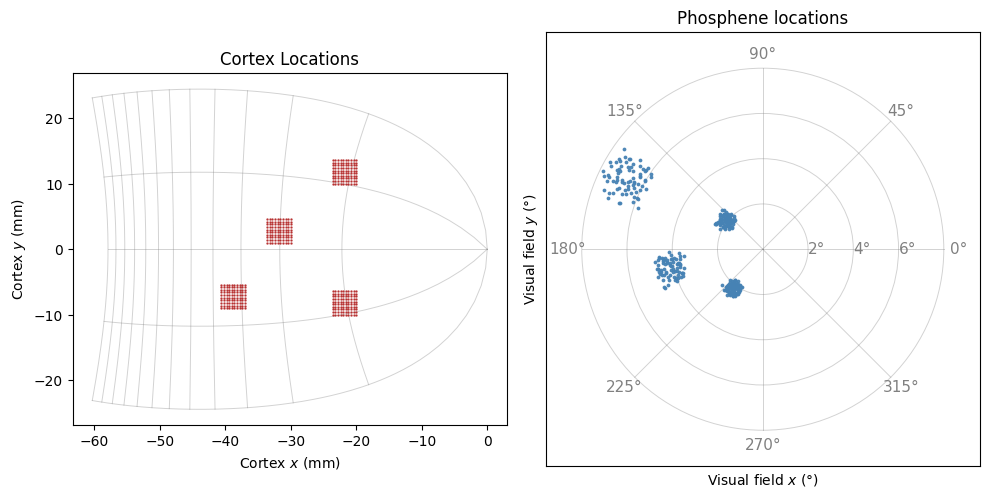
\includegraphics[width=0.9\columnwidth]{figures/cortextophosphenelocations4utaharrays.png}
  \caption{Cortical electrode locations of 4 Utah Arrays (left) plotted in cortical \(x,y\) coordinates with overlaid retinotopic grid, and corresponding phosphene centers (right) in visual‐field polar coordinates.}
  \label{fig:cortex-phosphene-locations}
\end{figure}

\subsubsection{Retinotopic Projection and Phosphene Centers}
Each cortical electrode \((x_i,y_i)\) is mapped into visual-field coordinates \((\mu_{x,i},\mu_{y,i})\) using the inverse of the Wedge–Dipole transform introduced by Polimeni \emph{et al.}\ \cite{Polimeni2006}. This model captures cortical magnification, in which the foveal region is allocated a larger cortical representation than the periphery. In complex notation the forward mapping from visual-field polar coordinates \((r,\theta)\) to cortical coordinate \(w\) is
\[
w = k\bigl[\ln\bigl(r\,e^{i\alpha\theta} + a\bigr) 
       - \ln\bigl(r\,e^{i\alpha\theta} + b\bigr)\bigr],
\]
where \(r\) is eccentricity in degrees, \(\theta\) is polar angle, \(k\) scales degrees to cortical millimeters, and \(a,b,\alpha\) are fitted parameters. Analytically inverting this relation yields
\[
r\,e^{i\alpha\theta}
  = \frac{b\,e^{\phi} - a}{1 - e^{\phi}},
\quad
\phi = \frac{w}{k},
\]
from which
\[
r = \bigl|\tfrac{b\,e^{\phi} - a}{1 - e^{\phi}}\bigr|,
\quad
\theta = \frac{1}{\alpha}\arg\!\bigl(\tfrac{b\,e^{\phi} - a}{1 - e^{\phi}}\bigr).
\]
Applying this inverse transform to each \((x_i,y_i)\) and adding optional Gaussian angular noise and dropout produces \(N\le E\) phosphene centers
\[
\{(\mu_{x,i},\mu_{y,i})\}_{i=1}^N,
\]
expressed in degrees of visual angle. These centers form the basis for SCAPE’s density estimation and adaptive filtering \cite{vanderGrinten2024}. An example implant scheme is shown in Figure~\ref{fig:cortex-phosphene-locations}, where the left panel plots the cortical electrode locations of 4 Utah Arrays in \(x,y\) coordinates and the right panel shows the corresponding visual‐field polar coordinates of the phosphenes.


\subsubsection{Gaussian Blob Rendering}
Empirical reports indicate that electrically evoked phosphenes are most often perceived as localized flashes of light with an approximately circular appearance \cite{vanderGrinten2024}. Although some studies describe elongated or irregular forms, for simplicity we model each phosphene as an isotropic Gaussian. Note that SCAPE’s core computations (density estimation and adaptive filtering) rely only on phosphene centers; the Gaussian shape is used downstream for visualization, evaluation, and amplitude normalization.

Formally, each phosphene center \((\mu_{x,i},\mu_{y,i})\) in visual‐field coordinates generates a two‐dimensional Gaussian blob
\[
G_i(x,y)
=
\exp\!\Bigl(-\frac{(x-\mu_{x,i})^2 + (y-\mu_{y,i})^2}{2\,\sigma^2}\Bigr),
\]
where \((x,y)\) are degrees of visual angle and \(\sigma\) is the nominal phosphene radius. The simulator rasterizes these Gaussians onto a regular image grid by converting \((\mu_{x,i},\mu_{y,i})\) into pixel positions according to the chosen field‐of‐view and resolution, evaluating \(G_i\) at every grid point, and summing across all \(N\) phosphenes:
\[
I_{\mathrm{raw}}(x,y)
=
\sum_{i=1}^{N} G_i(x,y).
\]
This raw phosphene map is then used for visualization, metric evaluation, and amplitude equalization but does not influence SCAPE’s density or filter‐scale computations. An example of this rendering is shown in Figure~\ref{fig:phosphene-rendering}, where the left panel plots the centers of the phosphenes in visual‐field coordinates and the right panel shows the corresponding Gaussian blobs.

\begin{figure}[h]
  \centering
  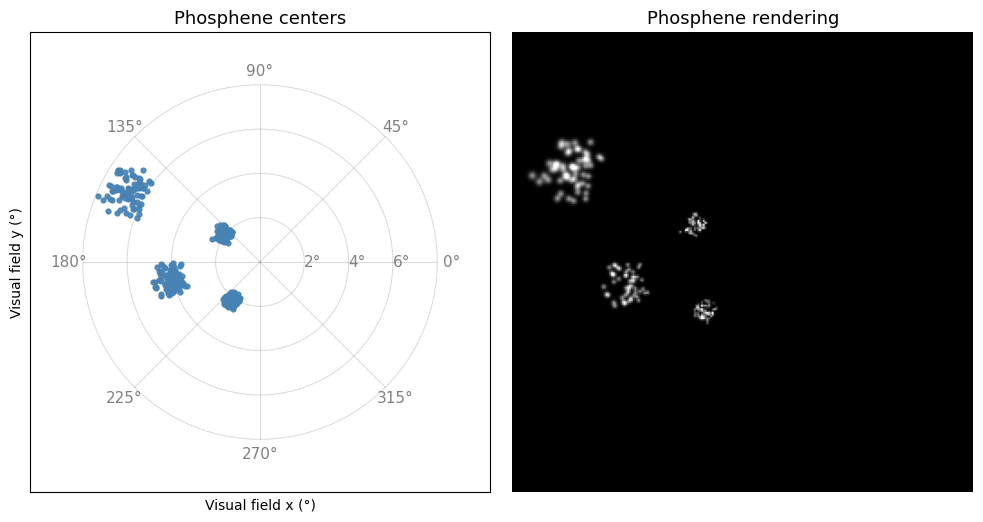
\includegraphics[width=0.9\columnwidth]{figures/phosphenerendering4utaharrays.png}
  \caption{Simulation of phosphene responses for a 4-Utah-array cortical implant. \textbf{Left:} Phosphene center locations in visual-field coordinates, shown on a polar grid spanning ±8° of eccentricity. \textbf{Right:} Corresponding Gaussian-blob rendering of phosphenes for a nominal stimulus amplitude (80 µA). This rendering illustrates how spatially discrete electrode activations translate into blurred perceptual spots that vary with cortical sampling density.}
  \label{fig:phosphene-rendering}
\end{figure}


\subsubsection{Activation-to-Electrode Mapping}

To evoke a specific percept with a cortical implant, we ultimately need to decide which electrodes to turn on and how much current to send through each.  A convenient intermediate representation is a continuous \emph{activation map} 
\[
  A(x,y)\in[0,1]
\]
defined over the visual field.  Intuitively, brighter regions of this map correspond to stronger intended stimulation, and darker regions to weaker or no stimulation.  

Given the $N$ electrode centers \(\{(\mu_i^x,\mu_i^y)\}_{i=1}^N\), we sample this map to produce a raw activation vector \(\mathbf{a}=(a_1,\dots,a_N)\).  Two common sampling strategies are:

\begin{itemize}
  \item \textbf{Point sampling:}  
    \(\displaystyle a_i = A(\mu_i^x,\mu_i^y)\).
  \item \textbf{Local pooling:}  
    \(\displaystyle a_i = \max_{(x,y)\in R_i} A(x,y)\), where \(R_i\) is a small neighborhood around \((\mu_i^x,\mu_i^y)\) (e.g.\ a disk whose radius reflects local magnification).
\end{itemize}

In our simulator implementation, we build a direct correspondence between each electrode and pixel(s) of the activation map by precomputing, for every electrode \(i\), a “distance map” on the visual‐field grid.  The simulator then uses these distance maps to (a) find the nearest pixel index for point sampling, or (b) define a binary mask for region pooling, entirely in pixel‐space.  

In a real implant system, the same correspondence can instead be obtained analytically: one applies the inverse retinotopic mapping (e.g.\ the wedge‐dipole transform) to compute exactly which image coordinates fall under each electrode’s receptive field, without requiring any precomputed pixel lookup.

Because \(A(x,y)\) was normalized into \([0,1]\), we then apply a global stimulus scale \(S\) (in Amperes) to obtain the actual per–electrode currents
\[
  I_i = S\,a_i.
\]
Choosing \(S\) appropriately ensures that we stay within safe charge‐delivery limits while preserving the relative pattern of activation.  This current vector \(\{I_i\}\) is then handed to the phosphene simulator, which applies temporal filtering, thresholding, and Gaussian‐blob rendering to generate the final perceptual image.  

In the end, our goal is to design or optimize the activation map \(A(x,y)\) (and thus the stimulus vector \(\{I_i\}\)) so that the resulting phosphenes are as clear and interpretable as possible.




\subsubsection{Amplitude Equalization}
Phosphene brightness does not scale linearly with electrode current. Local electrode density and current spread interact with multiple nonlinear stages, such as overlapping Gaussian-blob summation, saturation in sigmoid transforms, thresholding and temporal filtering, which cause some regions of the percept to appear disproportionately bright or dim. Because these nonlinear effects accumulate, there is no practical closed-form inverse that maps a target brightness profile back to electrode currents.

To achieve a uniform perceptual dynamic range, we apply a simple gain-learning step after simulation. Each phosphene \(i\) has an initial amplitude \(A_i=1\). We first drive all electrodes at the same nominal current \(S\), render the raw percept
\[
I_{\mathrm{raw}}(x,y)
=
\sum_{i=1}^N S\,G_i(x,y),
\]
and measure each blob’s peak intensity,
\[
m_i = \max_{x,y}\;G_i(x,y).
\]
We then optimize the gains \(\{A_i\}\) by minimizing
\[
\mathcal{L}(A)
=
\frac{1}{N}\sum_{i=1}^N \bigl(A_i\,m_i - m^*\bigr)^2,
\]
updating each \(A_i\) by gradient descent with learning rate \(\eta\) and clamping to \([A_{\min},A_{\max}]\). After convergence the normalized percept
\[
I_{\mathrm{norm}}(x,y)
=
\sum_{i=1}^N A_i\,S\,G_i(x,y)
\]
has phosphenes with comparable peak brightness, improving visual consistency for evaluation and downstream decoding.

\begin{figure}[ht]
  \centering
  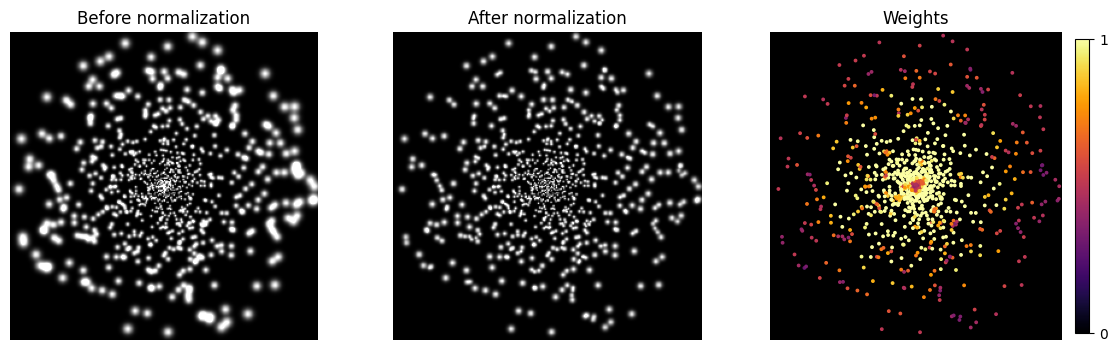
\includegraphics[width=0.9\columnwidth]{figures/dynamicamplitudenorm.png}
  \caption{Dynamic amplitude normalization example.  
    \emph{Left:} raw percept obtained by driving every electrode at the same current \(S\).  
    \emph{Center:} normalized percept after learning per-electrode gains \(A_i\).  
    \emph{Right:} learned gains \(A_i\in[A_{\min},A_{\max}]\).  
    Normalization yields a more even brightness profile and reduces total current draw, conserving implant power and minimizing excessive charge delivery.}
  \label{fig:amplitude_norm}
\end{figure}

This calibration step yields a more uniform perceptual phosphene map, improving clarity and interpretability of encoded images. Compressing the amplitude range also lowers the total current required, which reduces neural fatigue and extends implant battery life. Although amplitude equalization is not required by SCAPE’s core processing, we apply it here to standardize perceptual output for evaluation and comparison.



\subsection{SCAPE Adaptive Encoding}

The fundamental challenge in cortical prosthetic vision is that electrode arrays sample the visual field nonuniformly. Regions with dense electrode coverage can resolve fine detail while sparse regions cannot. SCAPE addresses this by adapting image filtering to the local sampling density. First, we estimate a continuous density map from the simulator-derived phosphene centers. Next, we convert density into a spatial scale map via sampling-theorem principles. Finally, we apply a shift-variant filter whose parameters vary continuously across the image. This adaptive encoding preserves maximal detail where it is supported and reduces visual clutter where it is not.

\begin{figure*}[ht]
  \centering
  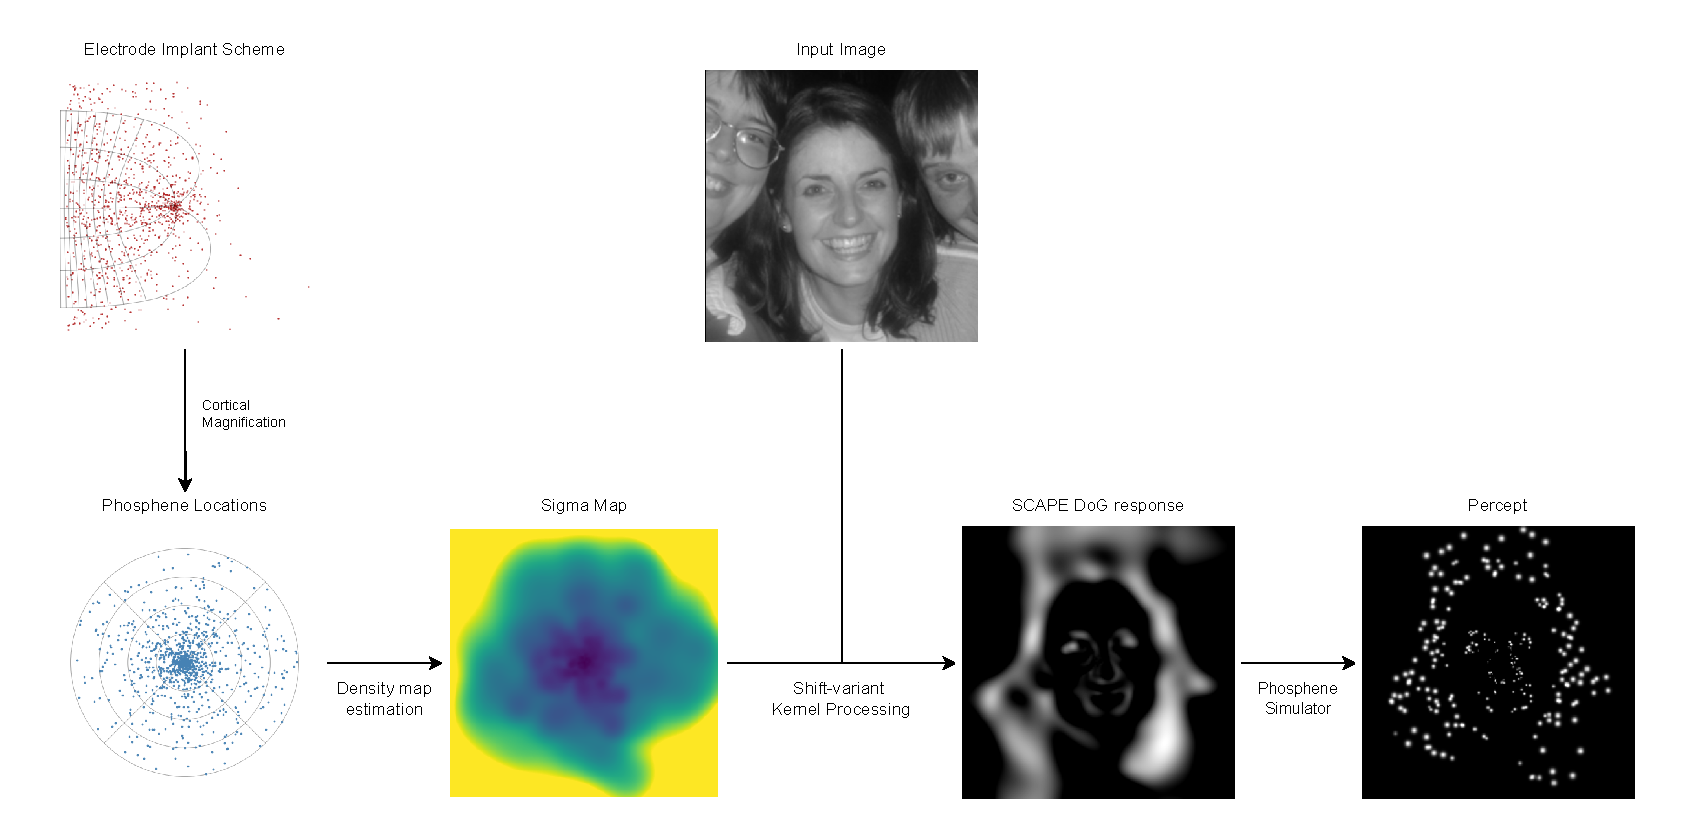
\includegraphics[width=\textwidth]{figures/SCAPElandscapeblack.pdf}
  \caption{Overview of the SCAPE pipeline. Starting from a cortical implant layout (top left) we obtain phosphene centers via the simulator, estimate a local density map, convert it into a spatial scale ($\sigma$) map, and then apply shift-variant filtering to produce an activation map for phosphene rendering.}
  \label{fig:scape_pipeline}
\end{figure*}

Figure~\ref{fig:scape_pipeline} illustrates the full SCAPE pipeline at a glance: from electrode layout to phosphene centers (Panel 1), to density and $\sigma$‐mapping (Panels 2–3), to the final shift‐variant filter output (Panel 4).  



\subsubsection{Density Estimation}
To guide adaptive filtering, SCAPE first computes a smooth sampling density \(d(x,y)\) over the visual field. This density reflects how densely the implant probes each region and sets the local spatial resolution limit. Two practical estimators are used.

\paragraph{Analytic Cortical Magnification}  
In an idealized implant that uniformly samples cortex around the fovea, one can predict density purely from known retinotopy. Writing eccentricity \(r=\sqrt{x^2+y^2}\) in degrees, the dipole‐model magnification  
\[
M(r)=\frac{k}{2\pi}\Bigl(\frac{1}{r+a}-\frac{1}{r+b}\Bigr)
\]
(with parameters \(k,a,b\) fit to human data \cite{vanderGrinten2024}) gives a nominal density  
\[
d_{\mathrm{analytic}}(x,y)=\frac{M(r)}{r}.
\]
We then scale \(d_{\mathrm{analytic}}\) so that its integral equals the total number of phosphenes \(N\):
\[
\iint d_{\mathrm{analytic}}(x,y)\,\mathrm{d}x\,\mathrm{d}y = N.
\]

\paragraph{Adaptive Kernel Density Estimation}  
For real implants with nonuniform phosphene layouts, we derive density directly from the simulator‐produced phosphene centers \(\{(\mu_{x,i},\mu_{y,i})\}\). We place a two‐dimensional Gaussian kernel at each center, choosing its bandwidth \(h_i\) based on local spacing. Specifically, let \(d_{(i,k)}\) be the distance from point \(i\) to its \(k\)th nearest neighbor; then
\[
h_i = \alpha\,d_{(i,k)},
\]
where \(\alpha\) (typically 1.0) controls smoothing. The density is
\[
d_{\mathrm{KDE}}(x,y)
= \sum_{i=1}^N \frac{1}{2\pi\,h_i^2}
\exp\!\Bigl(-\frac{(x-\mu_{x,i})^2 + (y-\mu_{y,i})^2}{2\,h_i^2}\Bigr).
\]
Finally we normalize so that
\[
\iint d_{\mathrm{KDE}}(x,y)\,\mathrm{d}x\,\mathrm{d}y = N.
\]
This adaptive KDE provides a flexible density estimate that captures local variations in electrode coverage.


\subsubsection{\(\sigma\)-Mapping via Nyquist Principles}
Once a smooth density map \(d(x,y)\) is available, SCAPE computes a spatial‐scale map \(\sigma(x,y)\) that indicates the precise local sampling limit. By the Nyquist sampling theorem \cite{Nyquist1928}, the highest spatial frequency resolvable at \((x,y)\) is
\[
f_{\mathrm{Nyq}}(x,y)
=\tfrac{1}{2}\sqrt{\frac{d(x,y)}{\pi}},
\]
since a local density of \(d\) phosphenes per unit area implies an average spacing of \(\Delta\approx\sqrt{1/d}\).  To match this limit exactly, we set
\[
\sigma(x,y)
= \frac{\kappa}{f_{\mathrm{Nyq}}(x,y)}
= 2\,\kappa\sqrt{\frac{\pi}{d(x,y)}},
\]
where \(\kappa>0\) (typically \(1\)) adjusts the transition sharpness.  The resulting \(\sigma\)-map directly specifies the standard deviation of the local processing kernel at each location, thereby guiding where and at what scale spatial frequencies should be preserved or suppressed.



\subsubsection{Shift-variant Filtering}
Having obtained a continuous filter‐scale map \(\sigma(x,y)\), SCAPE applies spatially adaptive filtering to the input image. At each location \((x,y)\), a local kernel \(K(\cdot;\sigma(x,y))\) is convolved with the image, yielding an output
\[
I_{\mathrm{filt}}(x,y)
=\iint K\bigl(u,v;\sigma(x,y)\bigr)\,
I_{\mathrm{in}}(x-u,y-v)\,\mathrm{d}u\,\mathrm{d}v.
\]
By tying the kernel’s parameters to the local sampling density, shift‐variant filtering preserves fine detail where electrodes are dense and reduces clutter where they are sparse. In the following sections we describe a concrete implementation using a difference of Gaussians and discuss how other kernel families can be incorporated within the same framework.


\paragraph{Difference-of-Gaussians Example}
As a concrete illustration of SCAPE’s adaptive filtering, we approximate the Laplacian-of-Gaussian (LoG) operator, widely used to model center–surround receptive fields in early vision \cite{Young1987}, with a pair of Gaussian kernels.  At each location \((x,y)\), the LoG of the input image \(I\) would be
\[
\mathrm{LoG}_{\sigma}(x,y)
=\nabla^2\bigl[G_{\sigma} * I\bigr](x,y),
\]
where \(G_{\sigma}\) is a Gaussian of standard deviation \(\sigma(x,y)\) and \(*\) denotes convolution.  Computing a full LoG at every pixel with its own \(\sigma\) has complexity \(\mathcal{O}(n^2)\) per pixel, where \(n\) is the kernel size, making it impractical for real-time use.  Instead, we approximate it by a Difference-of-Gaussians (DoG):
\[
\mathrm{DoG}_{\sigma}(x,y)
=\bigl[G_{\sigma_1} - G_{\sigma_2}\bigr] * I\,(x,y),
\quad \sigma_2 = \lambda\,\sigma_1,
\]
with \(\lambda>1\) (typically \(\lambda=1.6\)) chosen so that \(\mathrm{DoG}\approx\mathrm{LoG}\).

To implement this shift-variant DoG efficiently, we factor each Gaussian \(G_{\sigma}\) into separable one-dimensional kernels. This reduces the complexity to \(\mathcal{O}(n)\) per pixel and allows us to modulate kernel width dynamically according to the local \(\sigma(x,y)\) map.  In practice this involves two passes of row- and column-wise convolutions with varying standard deviations, yielding real-time performance even on mobile hardware.  This separable DoG serves as a simple yet powerful example of SCAPE’s core idea: by varying filter scale across the image, we capture fine edges where phosphene density is high and suppress noise where it is low.


\paragraph{Extending to Other Kernels}
While the DoG serves as a straightforward example, SCAPE’s shift-variant framework accommodates any spatial filter family.  For instance, one can replace the Gaussian kernels with orientation-tuned Gabor filters to emphasize contours aligned with cortical receptive-field preferences. More generally, the kernel \(K(\cdot;\sigma(x,y))\) may be parameterized by a small set of basis functions (wavelets, steerable filters) whose shape adapts with \(\sigma\).  In future work one can even learn these kernels end-to-end: by embedding SCAPE into a differentiable reconstruction pipeline, the per-location filter weights can be optimized jointly with a decoder network.  This flexibility allows SCAPE to capture both classical center–surround processing and more complex feature tuning while retaining its core principle of local, density-driven adaptation.  



\subsection{Reconstruction Decoder Integration}
Human perceptual evaluation of phosphene encodings requires extensive behavioral studies and cannot be conducted at scale. Phosphene images are also fundamentally different from natural scenes, being sparse assemblies of localized blobs rather than continuous luminance patterns. To approximate how much visual information survives encoding, we train a convolutional decoder to reconstruct the original scene from the phosphene map.

This decoder plays a role loosely analogous to downstream visual cortex: it must infer edges, textures, and object layouts from an abstract representation. Unlike the brain, however, the decoder can adjust all its parameters through gradient-based learning and is not constrained by biological priors. Despite these fundamental differences, a consistent improvement in reconstruction accuracy suggests that the encoding has preserved more of the scene’s essential structure.

Our protocol is based on the end-to-end autoencoder framework of de Ruyter van Steveninck et al.\ \cite{deRuytervanSteveninck2020}, but here we fix the encoder to SCAPE and train only the decoder. By comparing reconstruction error and perceptual feature losses under identical training conditions, we derive a quantitative measure of how readily SCAPE’s output can be interpreted, guiding future behavioral and clinical validation.  


\subsubsection{Attention-UNet Architecture}
The reconstruction decoder employs an Attention-UNet, an extension of the original U-Net \cite{Ronneberger2015} with integrated attention and channel-recalibration mechanisms. Key components include:

\begin{itemize}
  \item \textbf{Squeeze-and-Excitation (SE) blocks} to adaptively weight feature channels \cite{Hu2018}.
  \item \textbf{Dilated residual blocks} in the bottleneck for multi-scale context aggregation \cite{Yu2016}.
  \item \textbf{Spatial attention gates} on skip connections to emphasize salient regions \cite{Oktay2018}.
\end{itemize}

Down-sampling is achieved via max-pooling and up-sampling via transposed convolutions. A final 1×1 convolution with sigmoid activation produces a reconstructed grayscale image. This configuration balances context integration and selective feature focus, making it effective for recovering scenes from sparse phosphene representations.  



\subsection{Evaluation Metrics}
Comparing sparse phosphene encodings directly to natural images is inherently challenging, as conventional pixelwise measures assume dense, continuous luminance patterns. Nevertheless, low‐level fidelity metrics provide useful insight into structural preservation when applied carefully to upsampled phosphene maps. To obtain a more complete assessment, we combine these fundamental measures with representational similarity analysis, which evaluates the geometry of stimulus relationships, and decoder‐based reconstruction performance, which tests how accessible the encoded information is for downstream interpretation. Together, these complementary approaches offer a multifaceted evaluation of SCAPE’s ability to convey visual content through the phosphene bottleneck.

\subsubsection{Low‐Level Fidelity Metrics}
To quantify how faithfully SCAPE’s phosphene output \(I_p\) preserves the original scene \(I_o\), we apply full‐reference image quality metrics that each compute a local similarity or error map and then pool these values into a single score.  In the following paragraphs we describe how SSIM, VSI, MDSI and PIEAPP are formulated and computed for the pair \((I_p,I_o)\).  


\paragraph{Structural Similarity Index (SSIM)}  
The Structural Similarity Index \cite{Wang2004} evaluates local agreement in luminance, contrast, and structure.  At each pixel \((x,y)\) define
\begin{align*}
S_{\mathrm{SSIM}}(x,y)
&= \frac{2\,\mu_p(x,y)\,\mu_o(x,y) + C_1}
       {\mu_p(x,y)^2 + \mu_o(x,y)^2 + C_1}\\
&\quad\times
    \frac{2\,\sigma_{po}(x,y) + C_2}
         {\sigma_p(x,y)^2 + \sigma_o(x,y)^2 + C_2}\,,
\end{align*}
where all statistics are computed over a small window around \((x,y)\).  The overall SSIM is
\[
\mathrm{SSIM}(I_p,I_o)
= \frac{1}{M\,N}
  \sum_{x=1}^{M}\sum_{y=1}^{N}
  S_{\mathrm{SSIM}}(x,y).
\]


\paragraph{Spectral‐Residual Saliency Index (SR-SIM)}  
SR-SIM evaluates image fidelity by combining spectral‐residual visual saliency with gradient‐based structure similarity \cite{Zhang2012}.  Given a reference \(I_o\) and a phosphene image \(I_p\), let  
\[
\mathrm{SVRS}_o(x,y),\;\mathrm{SVRS}_p(x,y)
\]
be their saliency maps computed via the spectral residual of the log‐amplitude spectrum, and let  
\[
\mathrm{GM}_o(x,y),\;\mathrm{GM}_p(x,y)
\]
be their gradient magnitude maps (Scharr‐filtered).  We form two local similarity measures  
\[
S_{\mathrm{S}}(x,y)
=\frac{2\,\mathrm{SVRS}_o(x,y)\,\mathrm{SVRS}_p(x,y)+C_1}
      {\mathrm{SVRS}_o(x,y)^2+\mathrm{SVRS}_p(x,y)^2+C_1},
\quad
\]
\[
S_{\mathrm{G}}(x,y)
=\frac{2\,\mathrm{GM}_o(x,y)\,\mathrm{GM}_p(x,y)+C_2}
      {\mathrm{GM}_o(x,y)^2+\mathrm{GM}_p(x,y)^2+C_2},
\]
with constants \(C_1,C_2\) for numerical stability.  Defining  
\(\mathrm{SVRS}_m(x,y)=\max\{\mathrm{SVRS}_o,\mathrm{SVRS}_p\}\), the fused local score is  
\[
S_L(x,y)
=\bigl[S_{\mathrm{S}}(x,y)\bigr]\,
\bigl[S_{\mathrm{G}}(x,y)\bigr]^\alpha\,
\mathrm{SVRS}_m(x,y),
\]
where \(\alpha\) (typically 0.5) balances structure sensitivity.  The global SR-SIM index is the normalized sum  
\[
\mathrm{SR{\text -}SIM}(I_p,I_o)
=\frac{\sum_{x,y}S_L(x,y)}
      {\sum_{x,y}\mathrm{SVRS}_m(x,y)}.
\]
This metric captures both saliency‐weighted structural agreement and overall contrast fidelity in a computationally efficient manner.



\paragraph{Visual Saliency Induced Index (VSI)}  
VSI \cite{Zhang2014} augments structural similarity with a model of visual attention.  First, saliency maps \(v_o(x,y)\) and \(v_p(x,y)\) are computed for the reference \(I_o\) and phosphene image \(I_p\) using the SDSP spectral‐residual approach, which combines spectral residuals, spatial distribution and color cues to highlight regions likely to attract gaze.  These maps are normalized to the range \([0,1]\).  

Next, three local similarity maps are formed:
\begin{align*}
s_{\mathrm{vs}}(x,y)
&= \mathrm{sim}\bigl(v_o(x,y),\,v_p(x,y)\bigr),\\
s_{g}(x,y)
&= \mathrm{sim}\bigl(\nabla I_o(x,y),\,\nabla I_p(x,y)\bigr),\\
s_{c}(x,y)
&= \mathrm{sim}\bigl(C_o(x,y),\,C_p(x,y)\bigr),
\end{align*}
where \(\mathrm{sim}(a,b)=\frac{2ab + C}{a^2 + b^2 + C}\) is the standard similarity kernel, \(\nabla\) denotes the Scharr‐filtered gradient magnitude in luminance, and \(C_o,C_p\) are the two chromatic channels in a perceptual color space.  These maps are fused into a single local score
\[
S(x,y)
= s_{\mathrm{vs}}(x,y)\,\bigl[s_{g}(x,y)\bigr]^{\alpha}\,\bigl[s_{c}(x,y)\bigr]^{\beta},
\]
with empirically chosen exponents \(\alpha\) and \(\beta\).  Finally, a per-pixel weight
\[
W(x,y) \;=\;\max\!\bigl(v_o(x,y),\,v_p(x,y)\bigr)
\]
emphasizes salient regions.  The global VSI is the saliency‐weighted average:
\[
\mathrm{VSI}(I_p,I_o)
= \frac{\sum_{x,y}W(x,y)\,S(x,y)}
       {\sum_{x,y}W(x,y)}.
\]

\paragraph{Feature Similarity Index (FSIM)}  
The Feature Similarity Index (FSIM) evaluates image fidelity by comparing low‐level features known to align with human perception: phase congruency (PC) and gradient magnitude (GM) \cite{Zhang2011}.  Given a reference image \(I_o\) and a phosphene rendering \(I_p\), we first extract their PC maps \(\mathrm{PC}_o(x,y)\), \(\mathrm{PC}_p(x,y)\) and GM maps \(\mathrm{GM}_o(x,y)\), \(\mathrm{GM}_p(x,y)\).  At each pixel \((x,y)\) we compute two similarity measures:
\[
S_{\mathrm{PC}}(x,y)
= \frac{2\,\mathrm{PC}_o(x,y)\,\mathrm{PC}_p(x,y) + T_1}
       {\mathrm{PC}_o(x,y)^2 + \mathrm{PC}_p(x,y)^2 + T_1},
\quad
\]
\[
S_{\mathrm{G}}(x,y)
= \frac{2\,\mathrm{GM}_o(x,y)\,\mathrm{GM}_p(x,y) + T_2}
       {\mathrm{GM}_o(x,y)^2 + \mathrm{GM}_p(x,y)^2 + T_2},
\]
where \(T_1,T_2\) stabilize the ratios.  We then form a fused local score
\[
S_L(x,y)
= \bigl[S_{\mathrm{PC}}(x,y)\bigr]^\alpha\,
  \bigl[S_{\mathrm{G}}(x,y)\bigr]^\beta,
\]
with \(\alpha=\beta=1\).  Finally, FSIM weights each location by the maximal phase congruency  
\(\mathrm{PC}_m(x,y)=\max\{\mathrm{PC}_o(x,y),\mathrm{PC}_p(x,y)\}\), yielding
\[
\mathrm{FSIM}(I_p,I_o)
= \frac{\sum_{x,y}\mathrm{PC}_m(x,y)\,S_L(x,y)}
       {\sum_{x,y}\mathrm{PC}_m(x,y)}.
\]
This formulation emphasizes perceptually salient features while penalizing structural deviations between \(I_p\) and \(I_o\).


\paragraph{Mean Deviation Similarity Index (MDSI)}  
MDSI \cite{ZiaeiNafchi2016} assesses image fidelity by combining gradient and chromaticity similarities with deviation‐based pooling, making it robust to localized distortions.  Given a reference \(I_o\) and a phosphene image \(I_p\), let \(\nabla I_o\) and \(\nabla I_p\) be their gradient magnitude maps (computed via Prewitt filters) and let \(C_o, M_o\) and \(C_p, M_p\) be the two opponent color channels in a perceptual color space.  Define at each pixel \((x,y)\):  
\[
\mathrm{GS}(x,y)
= \frac{2\,\nabla I_o(x,y)\,\nabla I_p(x,y) + c_1}
       {\nabla I_o(x,y)^2 + \nabla I_p(x,y)^2 + c_1},
\qquad
\]
\[
\mathrm{CS}(x,y)
= \frac{2\bigl(C_o(x,y)\,C_p(x,y) + M_o(x,y)\,M_p(x,y)\bigr) + c_3}
       {C_o(x,y)^2 + M_o(x,y)^2 + C_p(x,y)^2 + M_p(x,y)^2 + c_3}.
\]
These maps are fused into a combined similarity
\[
S(x,y)
= \alpha\,\mathrm{GS}(x,y) + (1-\alpha)\,\mathrm{CS}(x,y),
\]
with weighting \(\alpha\).  To emphasize pixels where similarity deviates most from its mean, we compute  
\[
s_i = S(x_i,y_i)^{1/4}, 
\quad
\bar s = \frac{1}{N}\sum_{i=1}^N s_i,
\]
and pool by the Minkowski deviation
\[
\mathrm{MDSI}(I_p,I_o)
= \biggl[\frac{1}{N}\sum_{i=1}^N \bigl|\,s_i - \bar s\bigr|\biggr]^{1/4}.
\]
Deviations from the mean highlight regions where the phosphene encoding departs most from the reference structure, yielding a sensitive measure of localized fidelity loss.  
 

\paragraph{Content Loss}  
To capture perceptually meaningful differences beyond pixel‐wise errors, we measure the dissimilarity between deep feature representations of the phosphene image \(I_p\) and the original scene \(I_o\) extracted from a pretrained convolutional network.  Denote by \(\phi_\ell(I)\) the activation tensor at layer \(\ell\) of a VGG‐type model.  The content loss is then  
\[
\mathcal{L}_{\mathrm{content}}(I_p,I_o)
= \bigl\lVert \phi_\ell(I_p) \;-\;\phi_\ell(I_o)\bigr\rVert_2^2.
\]
By choosing mid‐ to high‐level layers, this loss emphasizes preservation of object structure and semantic content rather than low‐level textures \cite{Gatys2015,Zhang2018}.  In our experiments we normalize inputs using ImageNet statistics and extract features from VGG19, averaging across spatial dimensions to yield a single content‐distance score per image pair.  Lower content loss indicates that SCAPE’s encoding retains more of the high‐level scene layout that a human observer would deem important.  



\paragraph{Perceptual Image‐Error Assessment through Pairwise Preference (PIEAPP)}  
PIEAPP \cite{Prashnani2018} is a learned full‐reference metric designed to predict perceptual error by modeling human preferences between image pairs. It operates by decomposing the input images into overlapping patches and computing learned feature representations. Given a reference image \(I_o\) and a phosphene image \(I_p\), each patch \(k\) yields a feature embedding difference \(\Delta f_k\). A two‐stage regression network maps these differences to an estimated perceptual error \(d_k\in\mathbb{R}\) and an associated confidence weight \(w_k>0\). Formally, the model computes
\[
\Delta f_k = \varphi\bigl(P_k(I_o)\bigr)\;-\;\varphi\bigl(P_k(I_p)\bigr),
\]
where \(P_k(\cdot)\) extracts the \(k\)-th patch and \(\varphi\) is the learned feature encoder. The per‐patch perceptual error is then
\[
d_k = g\bigl(\Delta f_k\bigr),
\]
where \(g\) is a regression module that predicts the perceived dissimilarity. Weights are obtained as
\[
w_k = h\bigl(\Delta f_k\bigr),
\]
with \(h\) a second regression branch modeling reliability. The final PIEAPP score aggregates over all \(K\) patches:
\[
\mathrm{PIEAPP}(I_p, I_o)
= \frac{\sum_{k=1}^K w_k \, d_k}{\sum_{k=1}^K w_k}.
\]
This approach has been shown to correlate strongly with human judgments of perceptual error in natural images. In our experiments, we use PIEAPP as an approximate measure of perceptual fidelity by treating \(I_o\) as the original input image and \(I_p\) as the phosphene representation. Although PIEAPP was not trained on sparse phosphene patterns, lower scores still suggest that the encoding preserves more information relevant to human perception. For full details, see \cite{Prashnani2018} and the reference implementation.  


\subsubsection{Representational Similarity Analysis}
Representational Similarity Analysis (RSA) is a widely used framework in neuroscience for comparing the structure of internal representations across different systems \cite{Kriegeskorte2008}. Instead of requiring spatial alignment or direct correspondence between individual activation patterns, RSA abstracts each representation into a pairwise dissimilarity matrix. This approach enables comparisons across measurement modalities with very different spatial resolution and scales, such as fMRI voxel patterns, single-unit electrophysiology, and artificial neural networks.

In classic applications, each stimulus is represented as a vector \(r_i\) of activations in a brain region (for example, responses in V1). The representational dissimilarity matrix (RDM) is then defined by
\[
D_{ij} = \delta\bigl(r_i, r_j\bigr),
\]
where \(\delta\) is a dissimilarity metric such as correlation distance
\[
\delta_{\mathrm{corr}}(r_i, r_j) = \frac{1 - \mathrm{corr}(r_i, r_j)}{2}.
\]
This RDM characterizes how different the representations of all pairs of stimuli are relative to each other. 

Conceptually, RSA offers what Kriegeskorte et al. termed a "second-order" representational comparison: while first-order comparisons measure similarity between raw activations, second-order comparisons examine whether the geometric relationships between stimuli are preserved. In neuroscience, such second-order comparisons have been used to show that different cortical regions (e.g., V1 vs. higher visual areas) encode distinct relational structures that align with perceptual or semantic similarity \cite{Wang2018}.

This principle motivates our use of RSA for phosphene encoding. Phosphenes are, in a sense, direct artificial activations of V1. Although our encoding is constrained by electrode sampling, it still forms a structured response space, conceptually akin to biological V1 patterns. By building RDMs of phosphene renderings, we can ask whether the relational geometry of the stimulus space is retained. If it is, then different stimuli remain discriminable in the same way, even if their absolute fidelity is degraded.

Practically, for a set of \(N\) images, we flatten each phosphene rendering into a vector
\[
r_i = \mathrm{vec}\bigl(I_p(i)\bigr),
\]
and compute the correlation distance matrix
\[
D_p(i,j) = \frac{1 - \mathrm{corr}\bigl(r_i, r_j\bigr)}{2}.
\]
Similarly, we compute an RDM for the reference images \(I_o\). To quantify second-order similarity, we correlate the upper triangles of these matrices:
\[
\rho = \mathrm{corr}_{\mathrm{Spearman}}\Bigl(\mathrm{vec}\bigl(D_p^{\mathrm{upper}}\bigr), \,\mathrm{vec}\bigl(D_o^{\mathrm{upper}}\bigr)\Bigr).
\]
High \(\rho\) indicates that the pairwise relationships between stimuli are well preserved by the encoding, even if pixelwise error is high. Low \(\rho\) suggests that the encoding distorts the relational structure, potentially impairing discriminability.

Although we compute dissimilarities here in pixel space, RSA can be applied in any feature space. For example, one could use embeddings from a pretrained neural network (e.g., VGG activations), perceptual models, or even behavioral similarity judgments. This flexibility allows RSA to bridge low-level and high-level aspects of representation in a unified framework.

In summary, RSA enables us to quantify whether phosphene encodings retain the relative distinctions between stimuli: a property that is often more relevant for perception and recognition than absolute pixel fidelity alone.

\subsubsection{Reconstruction Performance}
As a final evaluation axis, we assess how effectively a decoder network can reconstruct the original input image from the phosphene representation. Unlike the low-level fidelity metrics applied directly to the phosphene maps, this approach yields reconstructed natural images, making it more appropriate to apply conventional perceptual and pixel-based quality measures.

Specifically, for each phosphene-encoded input, the trained decoder produces a reconstructed image \(\hat{I}_o\). We then compare \(\hat{I}_o\) to the original reference image \(I_o\) using a suite of complementary metrics. These include pixelwise measures such as mean squared error (MSE) and SSIM, as well as perceptual similarity metrics such as LPIPS, VGG-based perceptual distance, DISTS, and PIEAPP. For completeness, we also report advanced full-reference metrics including FSIM, MDSI, VSI, and SRSIM. Together, these scores provide a multifaceted view of how much visual detail the encoding preserves in a form usable for end-to-end reconstruction.

Because the reconstructions are natural images, these metrics are applied without further adaptation. Higher perceptual similarity and lower pixelwise error indicate that the encoding retains more information useful for reconstructing recognizable content.

\section{Experiments}
\label{sec:experiments}

The experiments are designed to evaluate how well SCAPE adapts to different visual scenes, implant layouts, and spatial sampling densities compared to non-adaptive baselines.  
We assess performance across multiple datasets with diverse image statistics and test a range of implant schemes that vary in electrode count and distribution.  
All methods are processed through the same prosthetic vision simulation framework to ensure a fair comparison.  
Performance is quantified using complementary approaches: low-level fidelity metrics applied to phosphene renderings, representational similarity analysis to assess preservation of stimulus relationships, and reconstruction-based evaluation to gauge how well a learned decoder can recover the original scene from each encoding.  
This multi-faceted evaluation allows us to capture both the structural accuracy of the encoded images and their potential usability for downstream perception.


\subsection{Datasets}
We evaluate SCAPE using three publicly available datasets chosen to span complementary domains of visual content and statistics that are relevant for prosthetic vision research:

\begin{itemize}
    \item \textbf{MS~COCO}: diverse natural scenes and everyday objects, providing varied spatial frequencies, textures, and complex layouts. This dataset serves as a benchmark for general-purpose encoding performance in uncontrolled environments.
    \item \textbf{LaPa}: human face images, representing structured, high-contrast features and smooth shading. Faces are particularly important for functional prosthetic vision, since face recognition and interpretation are critical for social interaction.
    \item \textbf{SUN}: indoor and outdoor scene photographs, ranging from cluttered to open environments. This dataset tests how well encoders generalize across large-scale scene structures and semantic diversity, which reflects the types of navigation and recognition tasks prosthesis users encounter in daily life.
\end{itemize}

All images are first converted to grayscale to reflect the fact that brightness is the dominant cue available in prosthetic vision, where phosphenes primarily convey intensity rather than color \cite{Wang2015}.  
In early visual cortex, luminance signals are more strongly represented than chromatic signals, making brightness the most relevant dimension for encoding.  
Preliminary experiments with color confirmed that intensity alone preserved the majority of task-relevant structure.

Grayscale conversion is performed using \textbf{Rec.\,709 perceptual luminance} (luma) weighting, which aligns with human brightness perception:
\begin{equation}
Y = 0.2126\,R + 0.7152\,G + 0.0722\,B,
\end{equation}
where $R$, $G$, and $B$ are normalized to $[0,1]$.  
After conversion, perceptual normalization is applied to ensure a consistent dynamic range across images before encoding.

\begin{table}[ht!]
\centering
\resizebox{\columnwidth}{!}{%
\begin{tabular}{lccc}
\toprule
Scheme & View angle (deg) & Electrodes ($N$) & Eccentricity range (deg) \\
\midrule
Uniform 1024  & 16.0 & 1024 & 0.001--7.984 \\
Neuralink     & 25.0 & 4224 & 0.000--12.095 \\
1 Utah array  & 0.4  & 94   & 0.009--0.203 \\
4 Utah arrays & 16.0 & 320  & 1.632--7.931 \\
\bottomrule
\end{tabular}%
}
\vspace{1em}
\caption{Implant layouts and basic properties. Counts reflect the effective number of electrodes inside the simulator field of view. Eccentricity is reported in degrees of visual angle.}
\label{tab:implant_schemes}
\end{table}


\subsection{Implant Schemes}
We evaluate SCAPE across four implant layouts that span large differences in sampling density, spatial extent, and geometric regularity. This set stresses density adaptation both in the foveal region and in the periphery, and it includes layouts used in recent prosthetic vision studies.

\paragraph{Uniform 1024}
This layout provides a dense, near-uniform sampling of the visual field and serves as a standard reference in the literature on differentiable prosthetic vision. It allows direct comparison to prior work that uses a similar order of magnitude in channel count \cite{deRuytervanSteveninck2020}. It also exposes whether SCAPE preserves fine structure when the density is sufficient across most of the field of view.

\paragraph{Neuralink shank}
This layout represents a high-site-count configuration that covers a wide field of view with thousands of closely spaced sites. Such arrays have been demonstrated in the Neuralink brain–machine interface platform, which integrates flexible polymer shanks with thousands of recording and stimulation channels \cite{Musk2019}. Related developments in ultraflexible electrode arrays further highlight the feasibility of maintaining long-term, high-density interfaces in cortical tissue \cite{Zhao2023}. Within our framework, this scheme stresses computational efficiency and scale selection, since local density varies strongly with eccentricity and along the shank geometry. It therefore provides a test case for whether SCAPE scales robustly to thousands of sites while maintaining stability and efficiency.

\paragraph{One Utah array}
This layout matches a single-array setup and concentrates sampling near fixation with a very small field of view. It reflects ongoing experimental configurations used in current research programs at the Institute of Bioengineering of the Miguel Hernández University. It tests SCAPE under severe channel limits and minimal coverage, which is useful for understanding performance in constrained early clinical or preclinical settings.

\paragraph{Four Utah arrays}
This layout models a realistic multi-array configuration with gaps between arrays and moderate channel count. It introduces strong spatial inhomogeneity due to array borders and inter-array spacing, which is a common feature of practical cortical implants. It therefore tests whether SCAPE can suppress clutter in sparse regions while preserving detail within array footprints.

\begin{figure*}[ht!]
    \centering
    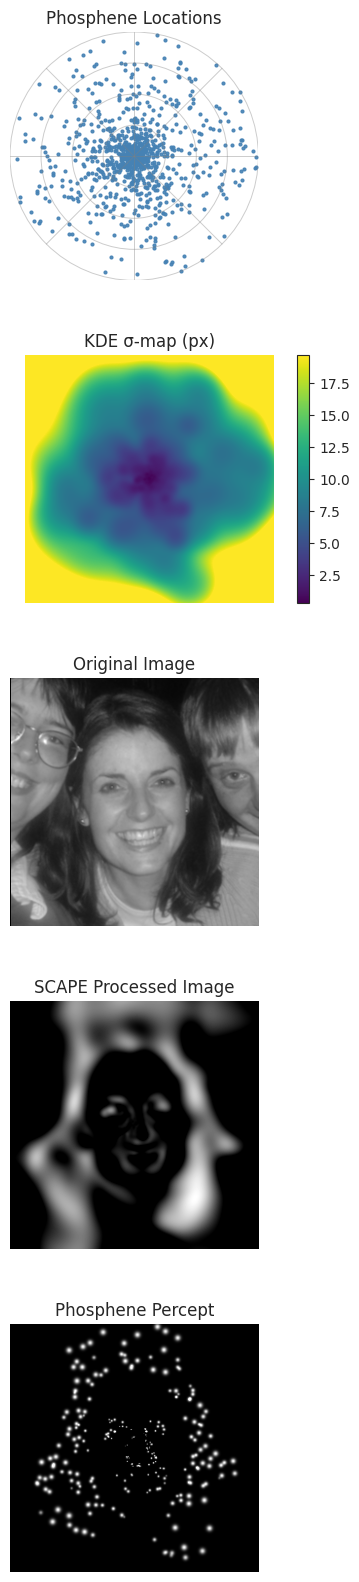
\includegraphics[width=0.23\textwidth]{figures/implant schemes/1024default.png}
    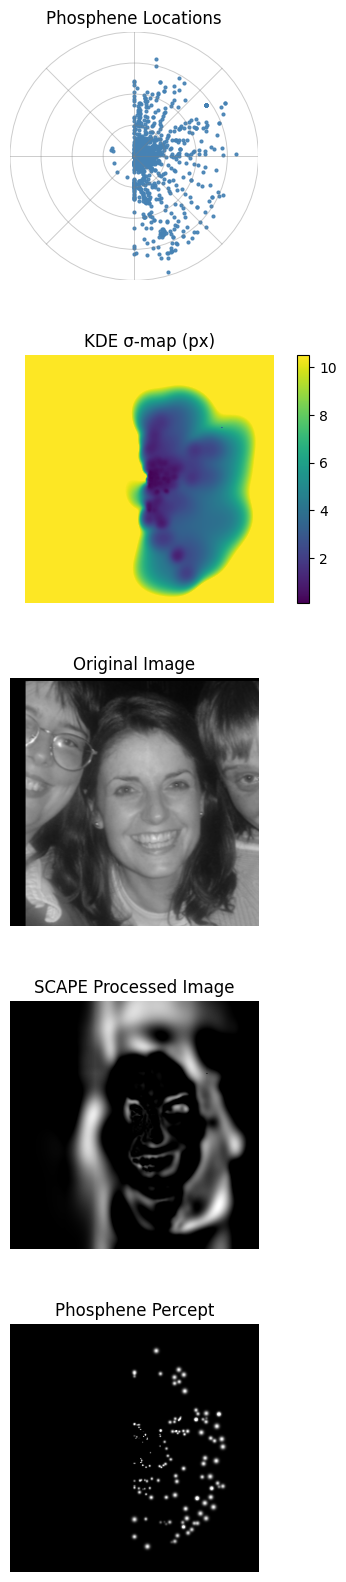
\includegraphics[width=0.223\textwidth]{figures/implant schemes/neuralink.png}
    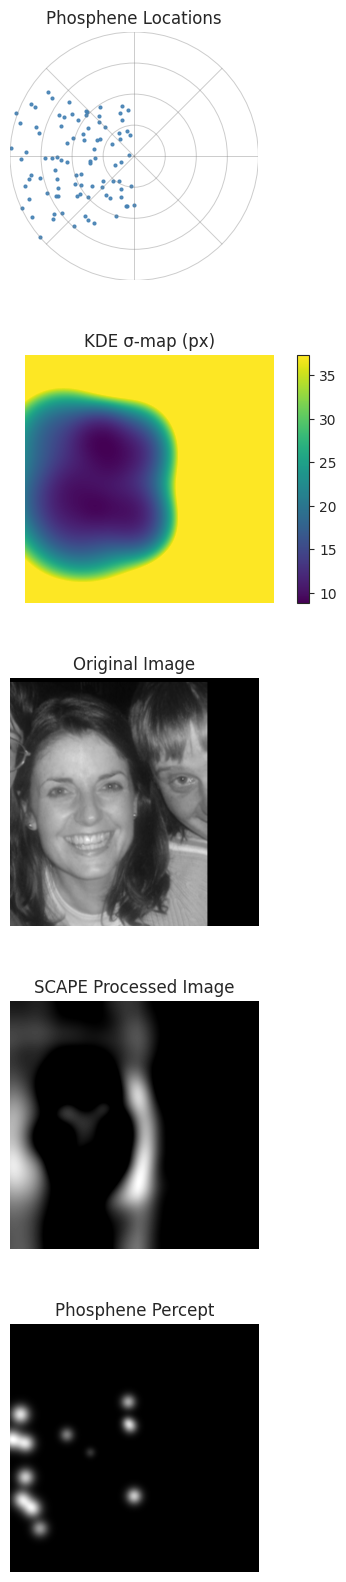
\includegraphics[width=0.223\textwidth]{figures/implant schemes/1 utah array.png}
    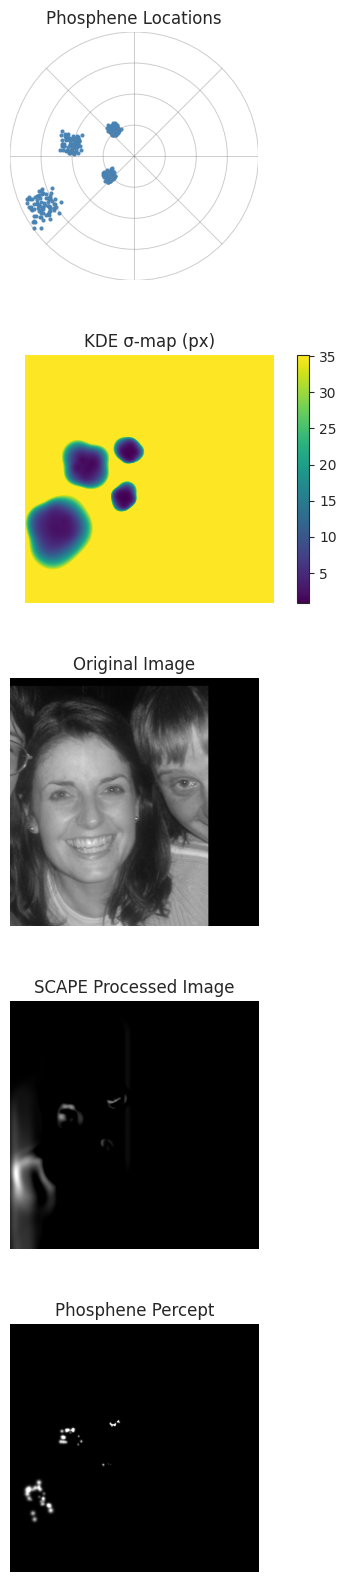
\includegraphics[width=0.223\textwidth]{figures/implant schemes/4 utah arrays.png}
    \caption{\textbf{Implant schemes used for evaluation.} 
    Each column illustrates one of the four electrode layouts tested in this study: Uniform 1024, Neuralink-type shank \cite{Musk2019,Zhao2023}, single Utah array, and four Utah arrays. For each scheme we show (top to bottom): electrode locations in visual field coordinates, the corresponding kernel density estimate (KDE) map of local sampling density, an example input image, the SCAPE-processed representation, and the resulting phosphene percept. The field of view differs between layouts and is scaled here for visualization. Together these schemes span large variations in electrode count, spatial distribution, and coverage, providing a diverse testbed for evaluating adaptive encoding.}
    \label{fig:implant_schemes}
\end{figure*}

\medskip
Together these schemes span two orders of magnitude in channel count, from 94 to 4224. They also span field of view from a fraction of a degree to more than twelve degrees of eccentricity. This diversity is important because SCAPE is designed to set filter scale from local sampling density. The chosen set probes that mechanism in both uniform and highly inhomogeneous layouts, which is essential for a fair test of adaptive encoding.


\subsection{Baselines}
We compare SCAPE against simple, widely used encoding strategies that do not adapt their spatial scale to local sampling density. Each baseline produces an activation map that is passed through the same simulator and amplitude normalization as SCAPE, ensuring that differences in outcome are attributable to the encoding strategy itself.  
Together, these baselines span a spectrum of encoding strategies: a contour-focused method (Canny), a bandpass but nonadaptive method (fixed DoG), and a structure-free random control.

\paragraph{Canny edge detection}
Canny edge maps are a standard choice in prosthetic vision pipelines because they preserve object boundaries under severe spatial resolution limits and often improve recognition in simulated conditions. We include a Canny baseline with standard smoothing and hysteresis thresholding, applied uniformly across the field of view. To enhance the visibility of extracted contours in the simulated percepts, edges are dilated with a $3 \times 3$ kernel \cite{deRuytervanSteveninck2020}. This baseline serves as a strong nonadaptive feature extractor centered on high-contrast contours.

\paragraph{Fixed-scale Difference of Gaussians}
We implement a fixed-scale Difference of Gaussians (DoG) filter as a second baseline. This method applies Gaussian smoothing at a fixed scale and subtracts it from the original image, producing a bandpass representation that emphasizes edges and local contrast. In contrast to SCAPE, the filter scale is uniform across the image and cannot adjust to local variations in sampling density or spatial frequency content. We use a fixed filter size of $\sigma = 3$, chosen to produce feature sizes comparable to the dilated Canny edges.

\paragraph{Random control}
As a structure-free control, we generate a random activation pattern that matches the total activation energy of the method under test. This ensures that any observed improvements are due to meaningful spatial structure in the encoding rather than trivial differences in overall current or luminance.

\begin{figure*}[ht!]
    \centering
    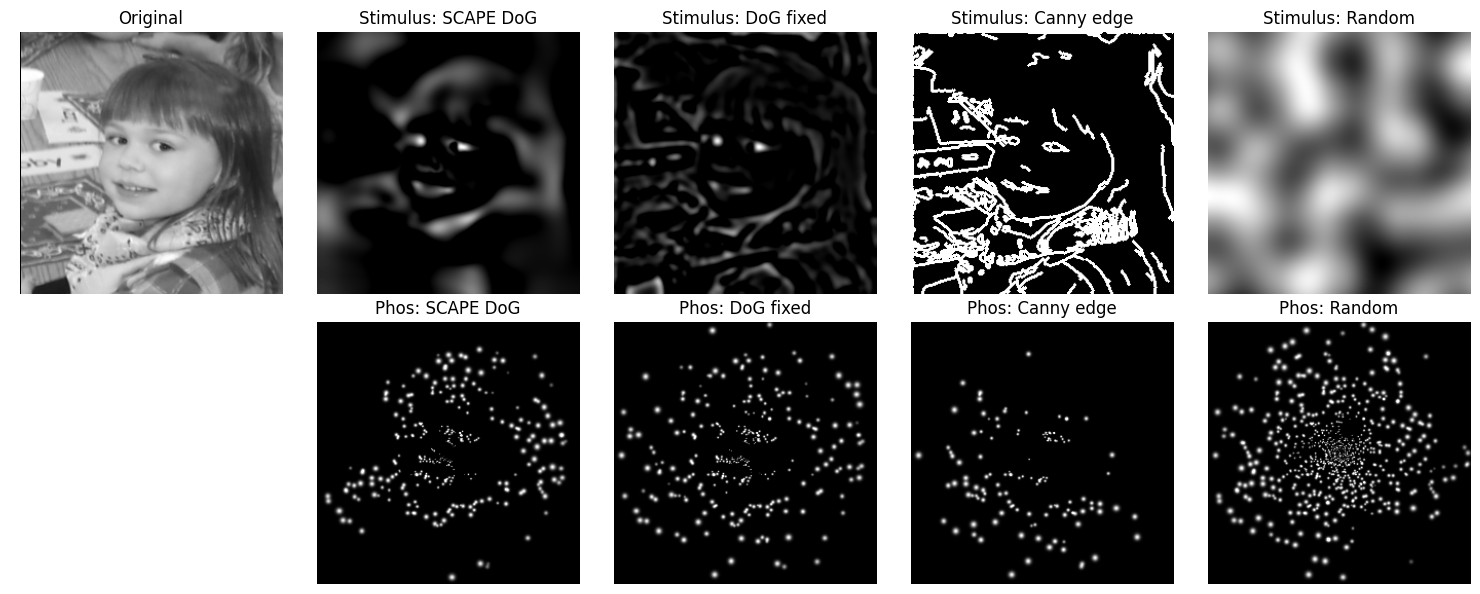
\includegraphics[width=\textwidth]{figures/processingmethods1.png}
    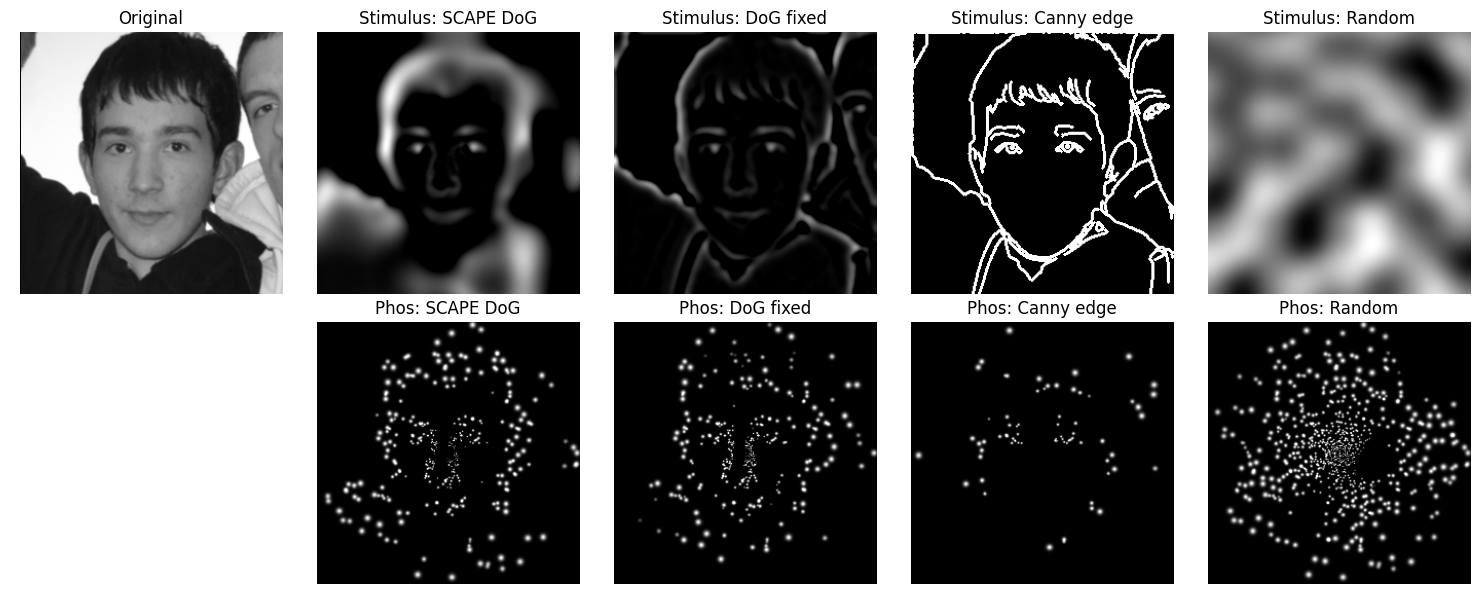
\includegraphics[width=\textwidth]{figures/processingmethods2.png}
    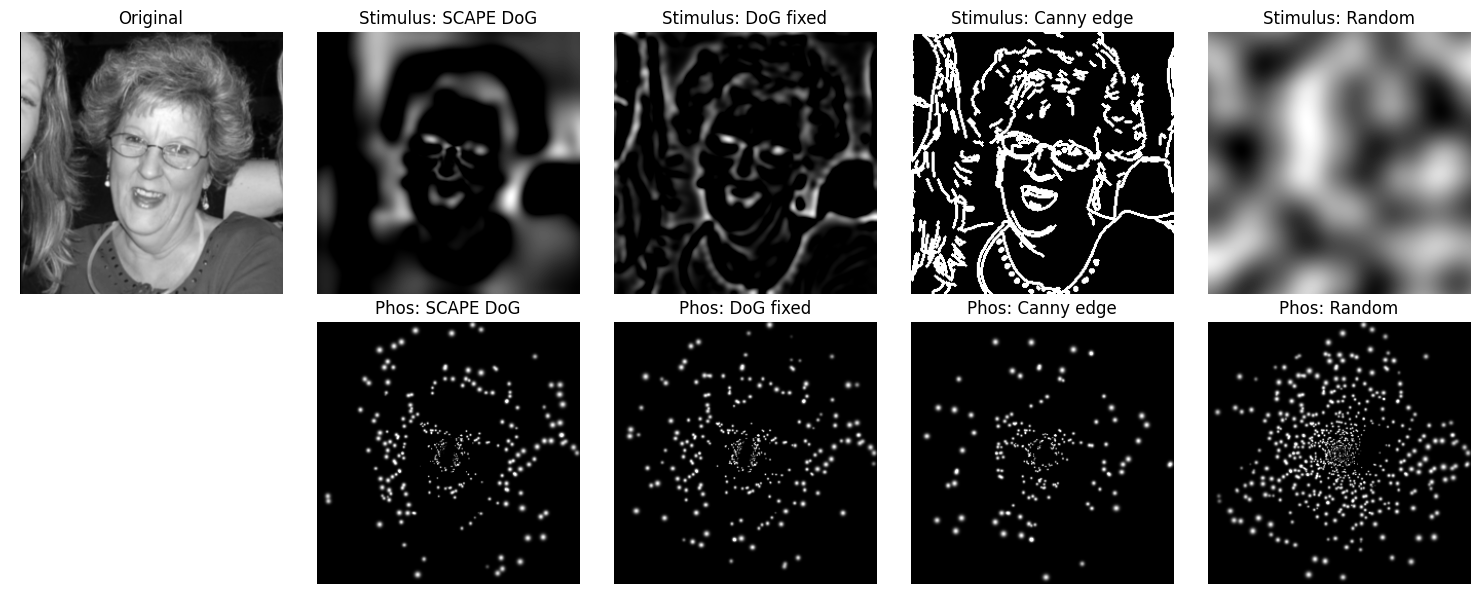
\includegraphics[width=\textwidth]{figures/processingmethods3.png}
    \caption{\textbf{Qualitative comparison of baseline and SCAPE encoders.} 
    Representative examples from the LaPa dataset. Top: stimulus representations after encoding. Bottom: corresponding phosphene renderings for the default implant scheme with 1024 electrodes. 
    SCAPE balances edge emphasis with adaptive clutter suppression, while fixed DoG and Canny either oversmooth or fragment the structure. Random activation patterns are added as a control.}
    \label{fig:qualitative}
\end{figure*}

\medskip
Representative examples of these baselines are shown in Figure~\ref{fig:qualitative}, together with SCAPE for comparison. All methods use identical preprocessing, simulator settings, and amplitude normalization, ensuring that differences in performance reflect only the encoding strategy rather than downstream rendering effects.

\subsection{SCAPE Configuration}
SCAPE builds a local density map from phosphene coordinates using adaptive kernel density estimation and converts that density into a spatial scale map \(\sigma(x,y)\). The scale map controls a shift variant Difference of Gaussians that runs with separable one dimensional passes.

\paragraph{Density estimation}
All experiments use adaptive KDE over phosphene centers in visual field coordinates. Bandwidth \(h_i\) for point \(i\) equals \(\alpha\) times the distance to its \(k\)-th nearest neighbor. We set \(k=16\) and \(\alpha=1.0\). The resulting density map is normalized so that its surface integral equals the total number of phosphenes of the scheme under test.

\paragraph{Mapping density to scale}
We convert density \(d(x,y)\) into a local scale through a Nyquist motivated rule. We use
\[
\sigma_{\text{fov}}(x,y) \;=\; \frac{2}{\pi \sqrt{2}\,\beta}\,\frac{1}{\sqrt{d(x,y)}} \quad\text{with}\quad \beta=0.55,
\]
which yields a scale that decreases in regions with higher sampling density and increases in sparse regions. For filtering on an image grid we convert \(\sigma_{\text{fov}}\) from degrees to pixels using the simulator field of view and resolution.

\paragraph{Stimulus alignment}
To ensure consistency across implant schemes, we center each input stimulus on the centroid of the \(\sigma(x,y)\) map. This alignment guarantees that the most informative regions of the stimulus overlap with the highest density regions of the implant layout, and it standardizes comparisons across schemes.

\paragraph{Filter family and execution}
We use a Difference of Gaussians with ratio \(\lambda=1.6\) to approximate a Laplacian of Gaussian while remaining efficient. The filter runs as two separable Gaussian passes per branch, first horizontal then vertical, at \(\sigma_1(x,y)\) and \(\sigma_2(x,y)=\lambda\,\sigma_1(x,y)\). Gaussian weights are truncated where their value falls below a small threshold and each one dimensional kernel is normalized to sum to one. Padding uses reflection at image borders. The half kernel radius is capped at a fixed maximum to bound runtime and memory.

\paragraph{Retinotopic model}
Retinotopic projection follows the dipole form of the Polimeni wedge–dipole family with standard parameters. This model sets the visual field coordinate system used by the KDE and by the degree to pixel conversion.

\paragraph{Sampling to electrodes}
The shift variant DoG produces an activation map on the simulator grid. Electrode currents are obtained by sampling the activation map at phosphene centers. The same sampling rule is used for every implant scheme.

\subsection{Amplitude Normalization}
To keep comparisons fair across encoders, we apply the same dynamic amplitude equalization to every method. The calibration runs once per implant scheme after mapping activations to electrode currents and before simulation. The resulting per electrode gains are reused for all images and all encoders within that scheme and across datasets. The procedure follows the definition in the Methods section and is tuned for stability.

We optimize the gains with a learning rate of \(0.002\) for \(2000\) steps, constrain each gain to \([0,\texttt{amplitude}]\), and use a small scale factor of \(1\times10^{-4}\) to set the update magnitude. In practice this removes simulator induced brightness bias, reduces extreme responses, and keeps total delivered current comparable, so the results reflect differences in encoding rather than artifacts of the simulation.

\paragraph{Representational similarity analysis}
For each dataset and implant scheme we construct representational dissimilarity matrices (RDMs) for the original images and for each encoded set. 
Each image is converted to a grayscale vector, and pairwise dissimilarity is computed as correlation distance
\[
D_{ij} = 1 - \mathrm{corr}(r_i, r_j).
\]
This produces an RDM that summarizes the relational structure of the stimulus set. 

To compare encoders, we correlate the upper triangular entries of the reference RDM with those of the encoded RDM using Spearman correlation \(\rho\). Higher \(\rho\) indicates closer alignment of relational geometry and thus better preservation of stimulus similarity structure. For visualization, we also report dissimilarity as \(1-\rho\), so that lower values correspond to better preservation. 

To obtain stable estimates, each method is evaluated on 500 randomly sampled images per dataset. Standard errors are estimated by 5000 bootstrap resamples, and statistical significance is assessed with 10{,}000 permutations. We report mean \(\rho\) (and \(1-\rho\) when plotting) per dataset and implant scheme for SCAPE and all baselines.


\paragraph{Reconstruction performance}
We measure how much scene information survives each encoding by training a fixed decoder to reconstruct the original image from phosphene renderings. For every encoder, dataset, and implant scheme we train an Attention U-Net on the corresponding phosphene maps using the same preprocessing, the same simulator settings, and the same training schedule. Inputs and targets are single-channel perceptual luminance images with the normalization described above. Evaluation uses a held-out split and reports MSE, SSIM, PSNR, LPIPS, DISTS, and VSI. Scores are computed per image and summarized as the mean with standard error. We also include representative reconstructions to illustrate qualitative differences that are not fully captured by the metrics.

For practical reasons we restrict reconstruction experiments to the Uniform 1024 scheme. Decoder training is specific to each implant layout, and running it for all schemes would multiply training cost substantially. The 1024 scheme provides a stable, widely used reference case in the literature and offers the fairest setting to compare encoders while keeping evaluation tractable.

\section{Results}
\label{sec:results}
\subsection{Qualitative Comparison of Encoders}
\label{sec:qualitative}

We begin by comparing encoders qualitatively to build intuition for their behavior before turning to quantitative analyses. 
Representative examples of SCAPE, fixed-scale DoG, Canny, and random control are shown in Figure~\ref{fig:qualitative} (see Section~\ref{sec:experiments}). 
Each method produces distinct patterns in both the encoded stimulus and the resulting phosphene rendering under the default 1024-electrode implant scheme.

Several systematic differences emerge. 
\textbf{SCAPE} emphasizes local contrast while suppressing spurious responses in low-density regions, yielding more interpretable percepts. 
\textbf{Fixed-scale DoG} captures edges but fails to adapt to varying density, leading to oversmoothing in dense regions and excessive detail in sparse ones. 
\textbf{Canny} extracts sharp contours but discards shading, resulting in fragmented and brittle percepts. 
Finally, the \textbf{random control} produces unstructured patterns with no relation to the input, serving as a sanity check. 

These qualitative examples illustrate why adaptive scale selection is important: SCAPE strikes a balance between edge emphasis and clutter suppression that is not achieved by fixed or contour-based baselines. The following sections quantify these observations using representational dissimilarity analysis and reconstruction performance.

\subsection{Representational Dissimilarity Analysis}
We next assessed the representational fidelity of different phosphene encoding strategies using RSA as defined in Section~\ref{sec:experiments}. 
Figure~\ref{fig:rsa_pixel} shows the dissimilarity of phosphene encodings relative to pixel-space RDMs across three datasets (COCO, LaPa, SUN) and four implant schemes. 
Lower values correspond to better preservation of the relational structure of the original images.

\begin{figure}[t!]
    \centering
    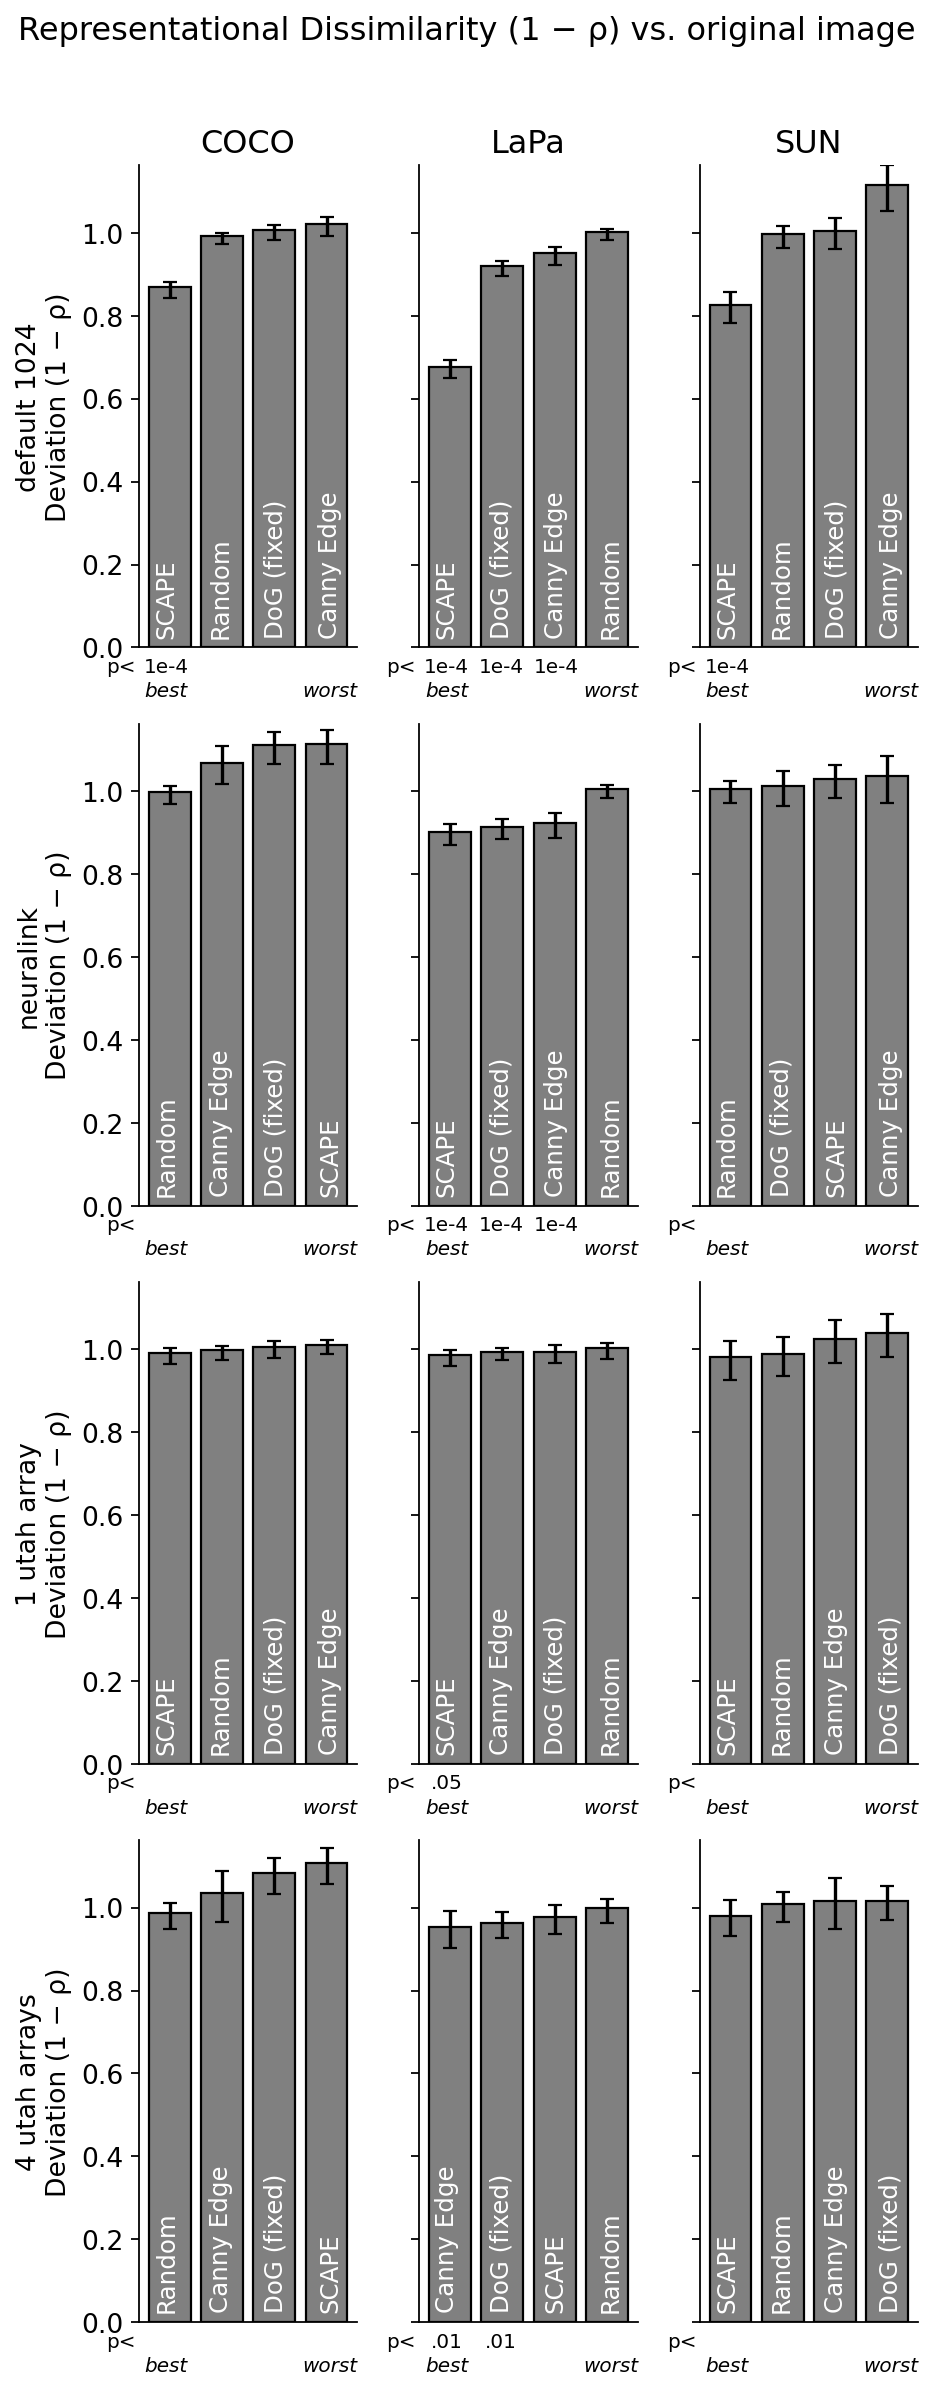
\includegraphics[width=0.9\columnwidth]{figures/RSA.png}
    \caption{\textbf{Representational similarity analysis relative to pixel-space reference.} 
    Dissimilarity ($1-\rho$) between phosphene encodings and original image RDMs across COCO, LaPa, and SUN datasets. 
    Bars show mean dissimilarity, error bars denote bootstrap confidence intervals, and $p$-values (permutation test) are reported below each bar. 
    Lower values correspond to greater preservation of pixel-space structure.}
    \label{fig:rsa_pixel}
\end{figure}

Across all conditions, \textbf{SCAPE (adaptive DoG)} achieved the lowest dissimilarity, indicating that its density-adaptive filtering preserves pixel-level similarity structure most effectively. 
The \textbf{fixed-scale DoG} baseline performed moderately well but failed to adapt across sampling densities, leading to higher dissimilarity in sparse layouts. 
\textbf{Canny edges} and the \textbf{random control} consistently produced substantially higher dissimilarities, reflecting poor alignment with stimulus similarity. 
Permutation-based $p$-values (shown below each bar) confirm that SCAPE significantly outperforms the nonadaptive baselines across datasets and implant schemes.


\subsection{Reconstruction Performance}
To complement the representational analysis, we evaluated how effectively a learned decoder could reconstruct natural images from phosphene representations. 
As noted in Section~\ref{sec:experiments}, reconstruction experiments were restricted to the Uniform 1024 scheme. 
Decoder training is specific to each implant layout, and running separate decoders for all schemes would multiply training cost substantially. 
The 1024 layout provides a stable and widely used reference case, making it the most appropriate benchmark for encoder comparison.

Quantitative results are summarized in Tables~\ref{tab:recon_coco}--\ref{tab:recon_sun}, grouped into intensity-based metrics (MSE, SSIM, PSNR) and perceptual similarity metrics (LPIPS, DISTS, MDSI, VSI).
Across all datasets, \textbf{SCAPE} consistently achieved the lowest MSE and the highest PSNR values, indicating superior fidelity in reproducing low-level intensities. 
SSIM scores showed a similar pattern on COCO and SUN, with more modest but consistent gains on LaPa. 
Perceptual metrics confirmed these findings: SCAPE generally outperformed the nonadaptive baselines across datasets, although individual metrics occasionally favored Canny (e.g., MDSI on COCO and SUN). 
Despite such cases, SCAPE provided the best overall balance across metrics, highlighting its robustness to diverse visual statistics.

Qualitative reconstructions further illustrate these trends. 
As shown in Figures~\ref{fig:recon_examples_coco}--\ref{fig:recon_examples_sun}, SCAPE reconstructions preserve continuous shading and object structure, enabling more interpretable outputs. 
By contrast, Canny emphasizes sparse contours at the expense of smooth surfaces, which often fragments object boundaries, while the random control produces severely degraded reconstructions lacking usable structure. 
Taken together, these results demonstrate that adaptive scale selection enables SCAPE to retain substantially more perceptually relevant information than nonadaptive encoding strategies. 
While decoder reconstructions are not direct behavioral measures, the ability to recover more naturalistic scenes suggests that human users may also benefit in perceptual and functional tasks, motivating future behavioral and clinical validation.


\begin{figure}[h]
  \centering
  \includegraphics[width=0.95\columnwidth]{/home/mappel/Dynaphos/spatial_frequency/results/DoG_coco/images/sample_0010.png}
  \includegraphics[width=0.95\columnwidth]{/home/mappel/Dynaphos/spatial_frequency/results/canny_coco/images/sample_0010.png}
  \includegraphics[width=0.95\columnwidth]{/home/mappel/Dynaphos/spatial_frequency/results/random_coco/images/sample_0010.png}
  \caption{Reconstruction examples on COCO under the Uniform 1024 scheme. Each row shows one encoding method: SCAPE (top), Canny edges (middle), and random control (bottom). Columns depict the pipeline from input image to activation map, phosphene rendering, and final reconstruction.}
  \label{fig:recon_examples_coco}
\end{figure}

\begin{figure}[h]
  \centering
  \includegraphics[width=0.95\columnwidth]{/home/mappel/Dynaphos/spatial_frequency/results/DoG_lapa/images/sample_0008.png}
  \includegraphics[width=0.95\columnwidth]{/home/mappel/Dynaphos/spatial_frequency/results/canny_lapa/images/sample_0008.png}
  \includegraphics[width=0.95\columnwidth]{/home/mappel/Dynaphos/spatial_frequency/results/random_lapa/images/sample_0008.png}
  \caption{Reconstruction examples on LaPa faces under the Uniform 1024 scheme. Each row shows one encoding method: SCAPE (top), Canny edges (middle), and random control (bottom). Columns depict the pipeline from input image to activation map, phosphene rendering, and final reconstruction.}
  \label{fig:recon_examples_lapa}
\end{figure}

\begin{figure}[h]
  \centering
  \includegraphics[width=0.95\columnwidth]{/home/mappel/Dynaphos/spatial_frequency/results/DoG_sun/images/sample_0008.png}
  \includegraphics[width=0.95\columnwidth]{/home/mappel/Dynaphos/spatial_frequency/results/canny_sun/images/sample_0008.png}
  \includegraphics[width=0.95\columnwidth]{/home/mappel/Dynaphos/spatial_frequency/results/random_sun/images/sample_0008.png}
  \caption{Reconstruction examples on SUN scenes under the Uniform 1024 scheme. Each row shows one encoding method: SCAPE (top), Canny edges (middle), and random control (bottom). Columns depict the pipeline from input image to activation map, phosphene rendering, and final reconstruction.}
  \label{fig:recon_examples_sun}
\end{figure}




\begin{table}[htbp!]
\centering
\scriptsize
\setlength{\tabcolsep}{2.5pt}   % tighter columns
\renewcommand{\arraystretch}{0.95}
\caption{Reconstruction metrics on the Uniform 1024 scheme across datasets (results restricted to Uniform 1024; see Section~\ref{sec:experiments} for rationale).}

\label{tab:recon_all}

\begin{subtable}{\columnwidth}
\centering
\captionsetup{font=footnotesize}
\caption{COCO}
\label{tab:recon_coco}
\resizebox{\columnwidth}{!}{
\begin{tabular}{lccc cccc}
\toprule
Processing model  & \multicolumn{3}{c}{Intensity reconstruction} & \multicolumn{4}{c}{Perceptual reconstruction} \\
\cmidrule(lr){2-4} \cmidrule(lr){5-8}
  & MSE & SSIM & PSNR & LPIPS & DISTS & MDSI & VSI \\
\midrule
SCAPE & \textbf{0.062} & \textbf{0.592} & \textbf{12.718} & \textbf{0.620} & \textbf{0.424} & 0.559 & \textbf{0.151} \\
Canny & 0.070 & 0.635 & 12.012 & 0.623 & 0.489 & \textbf{0.545} & 0.156 \\
Random & 0.071 & 0.635 & 11.999 & 0.695 & 0.636 & 0.600 & 0.179 \\
\bottomrule
\end{tabular}}
\end{subtable}

\vspace{0.5em}

\begin{subtable}{\columnwidth}
\centering
\captionsetup{font=footnotesize}
\caption{LaPa}
\label{tab:recon_lapa}
\resizebox{\columnwidth}{!}{
\begin{tabular}{lccc cccc}
\toprule
Processing model  & \multicolumn{3}{c}{Intensity reconstruction} & \multicolumn{4}{c}{Perceptual reconstruction} \\
\cmidrule(lr){2-4} \cmidrule(lr){5-8}
  & MSE & SSIM & PSNR & LPIPS & DISTS & MDSI & VSI \\
\midrule
SCAPE & \textbf{0.057} & \textbf{0.500} & \textbf{13.180} & \textbf{0.564} & \textbf{0.382} & \textbf{0.515} & \textbf{0.101} \\
Canny & 0.072 & 0.554 & 12.285 & 0.579 & 0.413 & 0.518 & 0.129 \\
Random & 0.076 & 0.566 & 12.003 & 0.625 & 0.516 & 0.560 & 0.147 \\
\bottomrule
\end{tabular}}
\end{subtable}

\vspace{0.5em}

\begin{subtable}{\columnwidth}
\centering
\captionsetup{font=footnotesize}
\caption{SUN}
\label{tab:recon_sun}
\resizebox{\columnwidth}{!}{
\begin{tabular}{lccc cccc}
\toprule
Processing model  & \multicolumn{3}{c}{Intensity reconstruction} & \multicolumn{4}{c}{Perceptual reconstruction} \\
\cmidrule(lr){2-4} \cmidrule(lr){5-8}
  & MSE & SSIM & PSNR & LPIPS & DISTS & MDSI & VSI \\
\midrule
SCAPE & \textbf{0.054} & \textbf{0.599} & \textbf{13.177} & 0.616 & \textbf{0.433} & 0.563 & \textbf{0.154} \\
Canny & 0.064 & 0.636 & 12.359 & \textbf{0.607} & 0.486 & \textbf{0.548} & 0.156 \\
Random & 0.067 & 0.638 & 12.171 & 0.676 & 0.582 & 0.602 & 0.189 \\
\bottomrule
\end{tabular}}
\end{subtable}
\end{table}
\section{Discussion and Conclusion}

\subsection{Summary of Contributions}
This work introduced SCAPE, a principled framework for encoding visual information in cortical prostheses that adapts spatial filtering to the local sampling density imposed by electrode layouts. Unlike conventional pipelines that apply uniform filters across the visual field, SCAPE derives a continuous density map from electrode or phosphene locations, converts this into a spatial scale map using Nyquist principles, and applies shift-variant filtering whose kernel width matches the local resolution limit. In an efficient implementation, we demonstrated a separable Difference-of-Gaussians operator that achieves real-time performance while preserving fine detail in dense regions and suppressing clutter in sparse regions.

Across multiple implant schemes and datasets, SCAPE consistently produced more interpretable percepts and preserved the relational structure of stimuli more effectively than nonadaptive baselines. Representational similarity analysis showed that SCAPE maintained pixel-space similarity geometry with higher fidelity, while reconstruction experiments revealed superior decoder performance on both intensity- and perceptual-based metrics. These improvements were observed consistently across natural scenes, faces, and indoor–outdoor environments, underscoring the robustness of the approach.

Together, these findings establish SCAPE as a general and efficient strategy for cortical implant encoding. By explicitly linking electrode density to filter scale, SCAPE provides a flexible foundation that can be integrated with existing simulators, extended with alternative kernel families, and adapted to patient-specific layouts. The framework therefore advances both the methodological toolkit for prosthetic vision research and the practical feasibility of density-aware encoding in future clinical systems.


\subsection{Relation to Prior Work}
The present work builds on several decades of research in prosthetic vision encoding while addressing a gap that has remained largely unfilled. Early heuristic pipelines emphasized contrast enhancement and edge extraction, which offered computational simplicity but treated the visual field uniformly. These methods were unable to balance the competing needs of preserving detail in regions of dense sampling and avoiding clutter where electrodes were sparse. More recent learned encoders have demonstrated that end-to-end optimization can improve perceptual quality, particularly when integrated with differentiable phosphene simulators. However, these approaches typically apply spatial filtering in a global manner, optimizing parameters across the full image rather than modulating them according to local sampling constraints.

SCAPE complements these earlier directions by introducing a middle ground between heuristic and fully learned solutions. Like heuristic methods, it is transparent, lightweight, and efficient, making it suitable for real-time use and hardware-constrained environments. At the same time, SCAPE is principled and general, deriving its adaptivity from electrode density and Nyquist sampling theory rather than hand-tuned heuristics. This makes it more systematic than early encoders and more interpretable than deep learned encoders, while remaining compatible with both paradigms.

Finally, SCAPE integrates naturally with recent differentiable simulation frameworks such as that of van der Grinten \emph{et al.}, which allow gradient-based optimization of encoders in realistic implant layouts. Embedding SCAPE into such pipelines enables hybrid approaches in which local density-driven filtering forms the initial encoding stage, while downstream networks can further refine or task-optimize the representation. In this sense, SCAPE provides a bridge between the transparency of heuristic designs and the flexibility of end-to-end learning, offering a principled foundation on which both research and clinical translation can build.

\subsection{Clinical and Practical Implications}
A central challenge in cortical prosthetic vision is that electrode arrays sample the visual field inhomogeneously. Uniform filtering strategies ignore this variation, often leading to oversmoothing in regions of high density and distracting clutter where coverage is sparse. By explicitly linking electrode density to filter scale, SCAPE addresses this mismatch and ensures that each region of the visual field is represented with the appropriate level of detail. This adaptivity has direct practical importance: it improves the interpretability of phosphene patterns, reduces spurious activations, and preserves fine structure where the implant supports it.

The benefits extend beyond simulated percepts. More faithful preservation of local structure implies that functional tasks such as object recognition, face perception, and scene navigation could become easier for users, since relevant features would remain distinguishable rather than being obscured by noise or excessive simplification. The strong performance of SCAPE reconstructions, especially on structured domains such as faces, suggests that the framework may support higher-level tasks critical for social interaction and daily functioning.

Equally important is the computational efficiency of SCAPE. The separable Difference-of-Gaussians implementation provides real-time performance on modest hardware, making the method compatible with the stringent latency and power constraints of implant systems. This efficiency ensures that the advantages of density-adaptive encoding are not merely theoretical but can be realized in practice on embedded devices and potentially integrated into future clinical systems.

Together, these properties position SCAPE as a practical foundation for next-generation cortical implant pipelines. By improving the clarity and usability of prosthetic percepts while remaining lightweight and transparent, SCAPE contributes to bridging the gap between laboratory simulations and clinical translation.

\subsection{Limitations}
While SCAPE provides a principled and efficient framework for adaptive phosphene encoding, several limitations should be acknowledged. First, all results were obtained in simulation. Although the simulator models important aspects of cortical stimulation and phosphene appearance, it cannot fully capture the variability and subjective experience of human percepts. Clinical evaluation will therefore be essential to validate whether the improvements observed in simulation translate into functional benefits for implant users.

Second, we evaluated usability indirectly through decoder reconstructions. Decoder performance offers a convenient proxy for how much visual information is preserved, but it is not equivalent to behavioral outcomes such as recognition accuracy, navigation performance, or reading speed. Direct psychophysical and clinical studies will be required to confirm that SCAPE leads to measurable improvements in real-world tasks.

Third, our analysis focused entirely on static images. We did not account for the temporal dynamics of stimulation, such as persistence, adaptation, or temporal integration of phosphenes. These dynamics strongly influence perceptual quality and functional performance in real use, and incorporating them into adaptive encoding remains an important direction for future work.

Finally, SCAPE is presented here as a heuristic grounded in sampling theory and density adaptation rather than as a fully optimized end-to-end solution. This makes it interpretable and efficient but also leaves open questions about how it compares to task-specific or learned encoders when evaluated in real use cases. Future behavioral experiments will be key to assessing the practical utility of SCAPE and to refining its role in clinical prosthetic vision pipelines.

\subsection{Future Directions}
Several avenues of research follow naturally from this work. A priority is to validate SCAPE in behavioral and eventually clinical settings. While simulation provides a controlled environment for development, only user studies can reveal whether the improved preservation of local structure translates into measurable benefits for recognition, navigation, and daily activities. Integrating SCAPE into immersive VR-based prosthetic vision platforms would provide a tractable next step toward such validation.

A second direction is to incorporate temporal dynamics of phosphene perception. The present study considered only static images, but in practice users encounter dynamic environments where persistence, adaptation, and temporal integration shape perceptual experience. Extending SCAPE to account for temporal structure—by adapting filter scale not only across space but also across time—may further improve perceptual clarity and stability.

Beyond these extensions, SCAPE offers a flexible foundation for hybrid approaches. Its density-driven filtering could be combined with human-in-the-loop optimization to tailor encoding to subjective reports, or integrated into differentiable pipelines where the adaptive filtering stage is refined jointly with a downstream decoder. More sophisticated kernel families, such as orientation-tuned Gabors or steerable filters, could also be explored to capture feature selectivity beyond isotropic contrast.

Finally, the computational efficiency of SCAPE makes it a promising candidate for deployment on resource-limited implant hardware. Future work should evaluate performance on embedded processors or FPGA-based platforms, ensuring that the benefits of adaptive encoding are practical under the latency and power constraints of clinical devices.

Together, these directions highlight how SCAPE can evolve from a principled static encoding framework into a broader platform that adapts across space, time, tasks, and hardware, ultimately supporting translation from simulation to patient use.

\subsection{Conclusion}
We introduced SCAPE, a density-adaptive framework for cortical prosthetic vision that links electrode layout to spatial filtering through Nyquist-based scale mapping. By implementing this principle with an efficient separable Difference-of-Gaussians, SCAPE preserves detail where electrode coverage is dense and suppresses clutter where it is sparse. Across multiple datasets and implant schemes, SCAPE consistently improved representational fidelity and reconstruction quality relative to nonadaptive baselines. These findings demonstrate that principled adaptation to local sampling density can substantially enhance the clarity and interpretability of simulated prosthetic percepts. SCAPE is lightweight, general, and compatible with existing simulators, making it well suited as a foundation for future patient-specific encoding strategies. By bridging the gap between heuristic efficiency and adaptive precision, SCAPE provides a promising step toward next-generation cortical implant pipelines and lays the groundwork for behavioral and clinical validation.


% ---- acknowledgments (if any) ----
% \section*{Acknowledgments}
% We thank…

% ---- bibliography ----
\bibliographystyle{plain}
\bibliography{references}

\end{document}
